%
% PROJECT: <ETD> Electronic Thesis and Dissertation Initiative
%   TITLE: LaTeX report template for ETDs in LaTeX
%  AUTHOR: Kayla Straub, kstraub@vt.edu
% SAVE AS: Straub_KM_T_2016.tex
% REVISED: February 17, 2016
% 


\documentclass[12pt]{report}

\usepackage{times}
\usepackage{graphicx}
\usepackage{amsmath}
\usepackage{amsthm, amssymb}
\usepackage{enumerate}
\usepackage{fullpage}
\usepackage{hyperref}
\usepackage{soul}
\usepackage{comment}
\usepackage{listings}
\usepackage{color} %red, green, blue, yellow, cyan, magenta, black, white
\definecolor{mygreen}{RGB}{28,172,0} % color values Red, Green, Blue
\definecolor{mylilas}{RGB}{170,55,241}
\usepackage{fancybox}
\usepackage{framed}
\usepackage{mathrsfs}
\usepackage{url}
\usepackage{paralist}
\usepackage{booktabs}
\usepackage[table]{xcolor}
\usepackage{floatrow}
\floatsetup[table]{capposition=top}
\usepackage[font=small,labelfont=bf]{caption}
\usepackage{fancyhdr} % Used for header
\usepackage[headsep=0.5cm,headheight=0.5cm]{geometry}
\usepackage{tocloft}
\hypersetup{breaklinks=true}
\urlstyle{same}
\usepackage[nottoc, numbib]{tocbibind}
\graphicspath{{Pictures/}}
\definecolor{Gray}{gray}{0.85}

\setlength\cftparskip{-2pt}
\setlength\cftbeforesecskip{1pt}
\setlength\cftaftertoctitleskip{2pt}

\setlength{\textwidth}{6.5in}
\setlength{\textheight}{8.5in}
\setlength{\evensidemargin}{0in}
\setlength{\oddsidemargin}{0in}
\setlength{\topmargin}{0in}

\setlength{\parindent}{0pt}
\setlength{\parskip}{0.25in}


\lstdefinelanguage{email}{
	basicstyle=\linespread{0.8}\scriptsize\color{black},
	keywordstyle=\color{black},
	identifierstyle=\color{black},
	stringstyle=\color{black},
	commentstyle=\color{black},
	breaklines=true,
	showstringspaces=false,%without this there will be a symbol in the places where there is a space
	numbers=none,%
	emph={},emphstyle=\color{black},
	frame=single,
	tabsize=4
}


% Uncomment for double-spaced document.
\renewcommand{\baselinestretch}{2}

\usepackage{epsf}

\begin{document}

\thispagestyle{empty}
\pagenumbering{roman}
\begin{center}

% TITLE
{\Large 
Data Mining Academic Emails to Model Employee Behaviors and Analyze Organizational Structure
}

\vfill

Kayla M. Straub

\vfill

Thesis submitted to the Faculty of the \\
Virginia Polytechnic Institute and State University \\
in partial fulfillment of the requirements for the degree of

\vfill

Master of Science \\
in \\
Electrical Engineering
\vfill

Robert W. McGwier, Chair \\
A. A. (Louis) Beex\\
R. Michael Buehrer\\
Bert Huang

\vfill

March 25, 2016 \\
Blacksburg, Virginia

\vfill

Keywords: Data analytics, machine learning, social computing
\\
Copyright 2016, Kayla M. Straub

\end{center}

\pagebreak

\thispagestyle{empty}
\begin{center}

{\large Data Mining Academic Emails to Model Employee Behaviors and Analyze Organizational Structure}

\vfill

Kayla M. Straub

\vfill

(ABSTRACT)

\vfill

\end{center}

Email correspondence has become the predominant method of communication for businesses.
If not for the inherent privacy concerns, this electronically searchable data could be used to better understand how employees interact. 
After the Enron dataset was made available, researchers were able to provide great insight into employee behaviors based on the available data despite the many challenges with that dataset.  
The work in this thesis demonstrates a suite of methods to an appropriately anonymized academic email dataset created from volunteers' email metadata.  
This new dataset, from an internal email server, is first used to validate feature extraction and machine learning algorithms in order to generate insight into the interactions within the center.  
Based solely on email metadata, a random forest approach models behavior patterns and predicts employee job titles with $96\%$ accuracy.
This result represents classifier performance not only on participants in the study but also on other members of the center who were connected to participants through email.
Furthermore, the data revealed relationships not present in the center's formal operating structure.
The culmination of this work is an organic organizational chart, which contains a fuller understanding of the center's internal structure than can be found in the official organizational chart.


\vfill

% GRANT INFORMATION


\pagebreak

% Dedication and Acknowledgments are both optional
\chapter*{Acknowledgments}
I want to acknowledge the many people who helped me with my graduate work at Virginia Tech and made this work possible.  Thank you to the members of my committee: Dr. Robert W. McGwier, Dr. Louis Beex, Dr. Michael Buehrer, and Dr. Bert Huang for your guidance.  In particular, I would like to sincerely thank Dr. McGwier for his vision and support throughout this research.  

I want to express my gratitude to the faculty, staff, and students of the Hume Center for all of your help and for providing me with the opportunities to work on such interesting research.  I am especially thankful for Dr. Joseph Ernst and Dr. William C. Headley for their invaluable insight and assistance.

I would also like to thank my family and friends for their support throughout my college career.  I want to specifically thank my husband Ben for his unwavering support and for always pushing me to be my best.

Finally, I thank God for all the blessings in my life and for getting me to where I am today.
\tableofcontents
\pagebreak

\listoffigures
\pagebreak

\listoftables
\pagebreak

\pagenumbering{arabic}
\pagestyle{myheadings}

\chapter{Introduction} \label{Introduction}
\section{Motivation}
A reorganization of a business can be very costly and has far-reaching effects once implemented, either for better or for worse.
While this official hierarchy is important, there is an equally important organic organization of any business, which may or may not be reflected in the official organization chart.
Understanding this unofficial structure could be invaluable during such a business reorganiztion, but due to its informal nature, it can be difficult to determine.
One massive source of electronically searchable information that could be used to better understand this hidden structure is the business's emails.
However, privacy concerns inhibit most research thrusts into email analysis.  

Extracting hierarchical relationships from email metadata can be used for several potential applications beyond gaining a better understanding of the organizational structure.  For example, it could be possible to identify people of influence or potential leaders.  By recognizing changing behavior, potential insider threats could be identified.

\section{Problem Overview}
This thesis addresses the problem of automatic organizational determination.
Specifically, it considers using email analysis to perform this operation.
However, there is a lack of modern, publicly available email datasets to use for this research.
Out of the email datasets that do exist, namely the Enron email corpus, there is a lack of accurate job title labels for the employees.
Labels are necessary for evaluating the results of the organic hierarchy analysis with the official organization chart.

The research presented in this thesis documents how a new email metadata dataset was collected and appropriately anonymized from the email records of 37 voluntary participants from an academic research organization.
This metadata is used not only to analyze the participants, but also to what extent the non-participant members of the organization can be characterized.


The problem of analysis is broken into two parts.
The first half addresses how to accurately classify employees by their job titles.
This will give insight into how well email behaviors indicate the official hierarchy as well as how similar the job titles are to one another.
The second part of the problem investigates how well this organic organizational chart matches the official organizational chart.
Altogether, the result reveals how much information about an organization can be extracted from the internal emails.



\section{Approach}
These emails are used to calculate a high-dimensional feature set to be used with machine learning techniques.
The 114 features used in this study can be grouped into two common areas in email analytics: traffic-based and social-based.
Using random forests, these features are used to accurately predict each employee's job title.
Finally, a comparison is presented between relationships displayed in the data with the formal organizational chart.
Combining predicted job titles with hierarchical relationships discovered from the data can identify an organization's true structure.

\section{Contributions}
The contributions outlined in this thesis show improvements to machine learning techniques applied to email analysis.  
First, a new, fully anonymized dataset was developed from raw emails from an academic research environment.  
This dataset, unlike others before it, has accurate job title labels.  
Furthermore, a unique combination of features was calculated from this data.  
Some had been used in email analysis before, but many are new and specific to this data.
Research investigating this problem in the past has focused on one of the two types of features, where this analysis aggregates traffic- and social-based features.
In general, the problem of job title classification has not been extensively studied.  
The leave-one-out cross-validation results in this thesis surpass the results of previous research on the Enron corpus.
Finally, a closer look at email relationships lends insight into the organic structure of the organization.


\section{Outline}
This thesis continues by discussing the related works in Chapter~\ref{PriorWork}.  
Chapter~\ref{Data} describes the process of data collection and some statistics of the dataset and the features extracted from the data.
The methods investigated using these features are covered in Chapter~\ref{Algorithm}.
The results of the analysis are presented in Chapter~\ref{Performance}.
 Chapter~\ref{FutureWork} presents opportunities for future work, and Chapter~\ref{Conclusions} concludes the thesis.


\chapter{Prior Work} \label{PriorWork}
This chapter investigates the previous research performed in the area of email analysis.
Context is established with a discussion on the importance of workplace email communication in modern society.
A description of the benchmark in email datasets, the Enron email corpus, is provided, and the drawbacks of this dataset are highlighted.
Section~\ref{sec:priorAnalysis} provides an overview of features typically used in email analysis and the works that address the problem of organization determination.

\section{Background}
Email is a pervasive medium for communication in modern society\textemdash{}particularly in the workplace.
In 2015, there were over 2.6 billion email users~\cite{radicati_emails_2015}.
It is projected that by the end of 2019, over one third of the global population will be using email.
In fact, the average business email user sends and receives a total of 112 emails per day.
Corporate email alone accounts for 54.7\% of worldwide email traffic.
Retention of large email archives has become common practice with decreasing memory size and cost~\cite{fisher_revisiting_2006}.
Out of the 600 employees involved in that study at Microsoft, the average employee had 28,660 emails stored in 133 folders; that represents a significant increase over the past ten years.
Such an accumulation of emails holds a considerable amount of untapped information that could be leveraged to characterize employee roles within an organization.

\section{Commonly Used Datasets} \label{sec:Enron}
When the Enron email corpus was released in 2004 \cite{klimt_introducing_2004}, it became the one of the largest email datasets available for public use.
It is unique in that it included all of the email text, which lead to many studies involving text analysis and natural language processing. 
Since then, this dataset has been extensively researched on topics including spam classification~\cite{bahgat2016mail}, \cite{shams_classifying_2013}; email categorization \cite{he_novel_2014}, \cite{keila_structure_2005}; and recipient prediction \cite{sofershtein_predicting_2015}, \cite{hu_towards_2012}.
However, there are known flaws and discrepancies with even the most recent versions of this dataset\textemdash{}ranging from misspelled email addresses~\cite{nordbo_data_2014} to duplicate email addresses~\cite{waterman_big_2014}, and misfiled emails~\cite{namata_inferring_2006}.
In one of the most popular forms of the dataset~\cite{shetty_enron_2004}, the database includes 253,735 emails sent as ``CC'' and  253,713 emails sent as ``BCC''.
Further inspection reveals that emails sent as one type or the other were almost always mistakenly recorded as both.

There exists a list of ground truth job title labels for the Enron email corpus~\cite{shetty_status_2004}, enabling corporate hierarchy analysis.
Previous work by Gilbert has made use of these labels along with performing natural language processing functions on the email text~\cite{gilbert_phrases_2012}.
This work identified phrases more likely to be used when emailing superiors compared to phrases used when emailing peers or subordinates.
The corpus and job title labels have also been used to explore patterns in office email gossip with respect to the organizational hierarchy~\cite{mitra_analyzing_2013}.
There are clear issues with the job title labels, though.
For example, Jeff Dasovic is labeled as an “Employee”, seemingly the lowest title.
However, he had more emails than anyone else in the dataset and is identified in records as “Director for State Government Affairs.” 
There are similar inconsistencies for Sally Beck, Rick Buy, and Rod Hayslett~\cite{gilbert_phrases_2012}.
Furthermore, out of the 161 employees with labels, 29 of them are listed as "N/A".
Amidst all of these concerns about the Enron job title labels, this work proposes using a new dataset with accurate job titles generated from intimate knowledge of the organization.

The other datasets for analysis are rare in this vein of behavior modeling and community analysis.
Other datasets used in the literature are usually either private or different types.
For example, the research by Tyler et al. was performed on a internal email dataset collected by HP labs that was not publicly released~\cite{tyler_email_2003}.
Often datasets collect communication patterns from public online sources such as Twitter~\cite{Zafarani+Liu:2009}, YouTube~\cite{mislove-2007-socialnetworks},  and Wikipedia~\cite{leskovec2010predicting}.
However, this research focused on organizational structure in addition to the social network components, so these datasets were unsuitable for this purpose.

\section{Prior Analysis} \label{sec:priorAnalysis}
The existing literature on analyzing social email behavior is mainly divided into two categories: traffic-based and social-based~\cite{tang_email_2013}.
Traffic-based methods calculate statistics based only on email patterns.
Social-based methods represent the email communications as a social graph and then extract information from this model about the inherent relationships.
A third type of feature that has been studied utilizes email text.
The work by Gilbert~\cite{gilbert2012phrases} showed that the wording used in an email could be used to make inferences about the corporate hierarchy.
However, email text contains sensitive information and is often unavailable for a general email study.
Therefore, features based on email text are not considered in this work.


By using features extracted from email metadata alone, previous work has been able to cluster levels of management at Enron~\cite{yelupula_social_2008}.
Other metadata features such as the presence of different email attachment types and the length of emails have been shown to successfully categorize email behavior~\cite{martin_analyzing_2005}.

For social-based features, relational ties can be modeled as a graph where nodes represent people and edges represent email interactions.
This is a useful model because many statistics can be calculated from the layout of a graphical layout~\cite{wasserman_social_1994}.
A common feature used in social network analysis is betweenness centrality, which comes in several different flavors, first developed by Freeman~\cite{freeman_set_1977}.
Betweenness centrality is a measure of how many shortest paths in a graph travel over each node.
In a graph with edge weights, as will be used in this work, a shortest path is a route from one node to another that has the minimum edge weight sum.
Note that two or more equivalent shortest paths can exist for a pair of nodes.
A node with high betweenness centrality in a social graph has been shown to represent a high degree of influence on other nodes.
A betweenness centrality algorithm has been used to determine community structures within an organization~\cite{tyler_email_2003}.
There are several other types of centrality such as degree, closeness, current-flow closeness, and current-flow betweenness~\cite{balinsky2011rapid}.
Avrachenkov et al. evaluated variations of betweeness centraltiy on the Enron dataset and other social networks~\cite{avrachenkov2013alpha}.
Furthermore, Agrawal et al. classified Enron employees within superior-subordinate pairs.
Using degree centrality features generated more accurate labels than natural language processing methods~\cite{agarwal_comprehensive_2012}.
Other research has detected the most important email users within a corporate network without using betweenness or centrality as features~\cite{wilson_discovery_2009}.
Examples of alternative features include: degree, the number of edges connected to a node; density, the ratio of actual edges to the number of possible edges; and proximity prestige, the ratio of the number of nodes that can reach a node $i$ to the average distance from those nodes to $i$.

Instead of considering exclusively traffic-based or social-based analytics, these feature types can be be used jointly.
The only example of this approach combined features such as number of emails, response time, cliques, and degree centrality into a ``Social Score'', was used to rank Enron employees~\cite{rowe_automated_2007}.  
Unfortunately, this work represents preliminary research and did not publish any quantifiable results.
This thesis aims to expand on this work and quantify the results when applied to a new dataset.

\chapter{Email Dataset and Feature Extraction} \label{Data}

This chapter details all of the steps taken to transform the raw data into the high-dimensional feature space used in the learning algorithm.
Information is provided on the data collected and statistics about the dataset.
There is a detailed description of all features used, both traffic-based and social-based.

\section{Data Collection}
Over the past decade, the Enron dataset has been widely used to study email behaviors because it is one of the only datasets available comprised of real-world corporate emails.
A list of ground truth job titles is available~\cite{shetty_status_2004}, however there are known issues with these labels.
Due to difficulties with the Enron dataset, as described in Section~\ref{sec:Enron}, this study uses a new dataset generated from emails provided by volunteers from one of the university's centers.

In consideration of the inherent privacy concerns, it was necessary to work with the Internal Review Board (IRB) to approve a data collection process which maintains participants' privacy.
This dataset is meant to be representative of metadata which any company could use without divesting employees of their email privacy.
Special care was taken to protect the privacy of those involved in the study.
During the collection process, all subject and body text was hashed using the MD5 algorithm.
A hashing algorithm was used to protect the email text of the participants because once text is hashed, it is impossible to recover the original message.
An example hash is shown in Figure~\ref{fig:hash_ex}.
All email metadata was stored in a MySQL database using scripts without any researchers observing any email text.
Any identifying information has been omitted from this thesis.
No unauthorized persons had access to the database, which was stored on a password-protected server run by the center.
\begin{figure}[t]
	\centering
	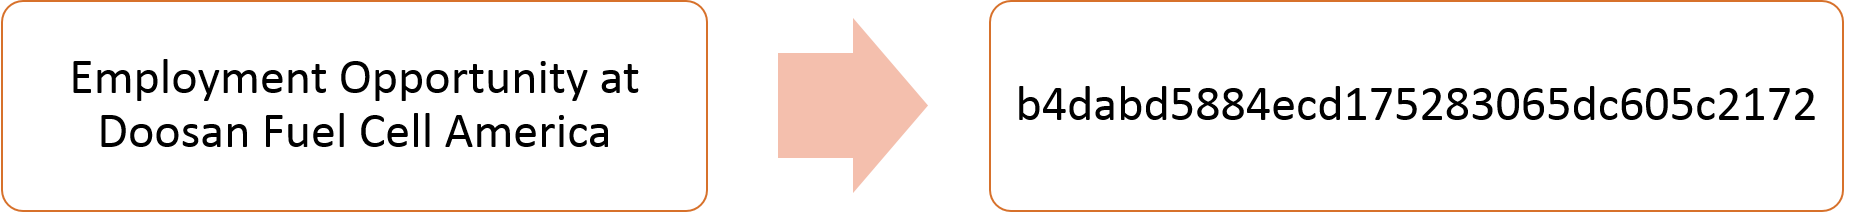
\includegraphics[width=\columnwidth,trim={0mm 0mm 0mm 0mm},clip]{hash_ex}
	\caption[Example subject hash]{The subject on the left was hashed using the MD5 algorithm to obtain the string on the right.  Hashing algorithms only function in one direction such that the original text cannot be recovered from the hashed string.}
	\label{fig:hash_ex}
\end{figure}


The first step in the data collection process was to design an accurate automated email parser.
This script would extract the metadata from raw emails.
Email formats can vary based on clients used or whether the email was sent from a mobile phone, which meant the parser script needed to be generic enough to handle many different configurations.
Small issues included recognizing forwarded emails as any of the following subject prefixes: "Fw:", "Fwd:", or "FW:".
The biggest obstacle was handling emails with embedded HTML.
For each email, the parsing script first needed to recognize that there was HTML present in the body text, then accurately parse the information from the tags.
Attachments were also difficult to handle because they appeared as immense blocks of encoded text.
The parser was designed to identify attachments and not include that text in the character count.  
An example email with both HTML and an attachment is in Appendix A.

Most of the collected data is information from the header of an email such as the sending and receiving email addresses and date and time.
The number of characters in the subject and body text were extracted before the subject and body text was hashed.
The prefix of the email was also recorded before hashing.
The hashed body and subject were loaded into the database in order to discern between emails with the same text.
For example, if an email is forwarded, it will have the same hashed subject once the prefix is removed, and it is therefore possible to count the number of times an email with the same subject has been received.
The number of attachments to each email was also collected.
The center's email server offers the ability to both digitally sign and encrypt emails.
Sending an email with either or both of these options appears as a special type of attachment in the raw email file.
Therefore, during the data collection process, information about whether an email was signed or encrypted was recorded.  All of the metadata was collected by a comprehensive parser script.  The types of information extracted from each email are:
\begin{itemize}
	\setlength\itemsep{-0.75em}
	  
	\item Destination and source email address    
	\item Email time stamp                        
	\item Subject prefix (e.g., Re:, Fwd:)        
	\item Hash of subject after removing prefix   
	\item Hash of body text                       
	\item Length of subject in characters         
	\item Length of body text in characters       
	\item Number of attachments                   
	\item Indicator if email was digitally signed 
	\item Indicator if email was encrypted        

\end{itemize}



\section{Dataset Description and Statistics}
Table~\ref{tab:db_stats} compares statistics between this internal dataset and the Enron corpus.
This internal database is more modern, contains more emails, and covers a longer time period, but it involves fewer people than were used to construct the Enron dataset.
While the study collected email data from only $36$ volunteers, the email metadata from these volunteers identified $38$ additional employees of the center.
These peripheral employees were included in the study when ground truth for their job was available and when the dataset contained sufficient email metadata records (defined as at least $100$ total emails).
Five of the $36$ direct participants were very new employees to the center, and are not considered in the classification analysis due to lack of sufficient email data.
The email records provided by these employees were still included to help characterize other employees.
Therefore, for all analyses in Chapter~\ref{Performance}, a total of $69$ people were classified, and this set is comprised of $31$ primary participants and $38$ peripheral employees.

\begin{table}[t]
\centering
\caption{A comparison between the internal dataset and the Enron email corpus.}
\label{tab:db_stats}
\resizebox{0.7\textwidth}{!}{%
\begin{tabular}{@{}lrr@{}}
\toprule
                   & Center          & Enron         \\ \midrule
Time               & Nov. 2012 - Nov. 2015     & Jan. 2000 - Sept. 2002 \\
Distinct Email Addresses & 32,030          & 75,406        \\
Participants       & 36              & 158           \\
Distinct Emails    & 579,594          & 252,759       \\ \bottomrule
\end{tabular}
}
\end{table}

Figure~\ref{fig:emails_over_time} shows the email traffic of the center over time.
The growth of the center between early 2013 and late 2015 is evident by the increasing baseline email traffic.
Note that each year before February is a dip in email activity.
This is indicative of Virginia Tech's winter break and Christmas holidays.
The spikes in the graph, such as in July 2013 and February 2014, and denote when email inboxes of employees were migrated from an old mail server.
For the first year of the new mail server, emails were copied over using a script which changed the timestamp of the emails to the time when they were copied.
These emails were not removed from the database, however, because they represent important interactions between center employees.
A more sophisticated migration process was implemented during the summer of 2014, which reduced the occurrence of such spikes.


\begin{figure}[t]
	\centering
	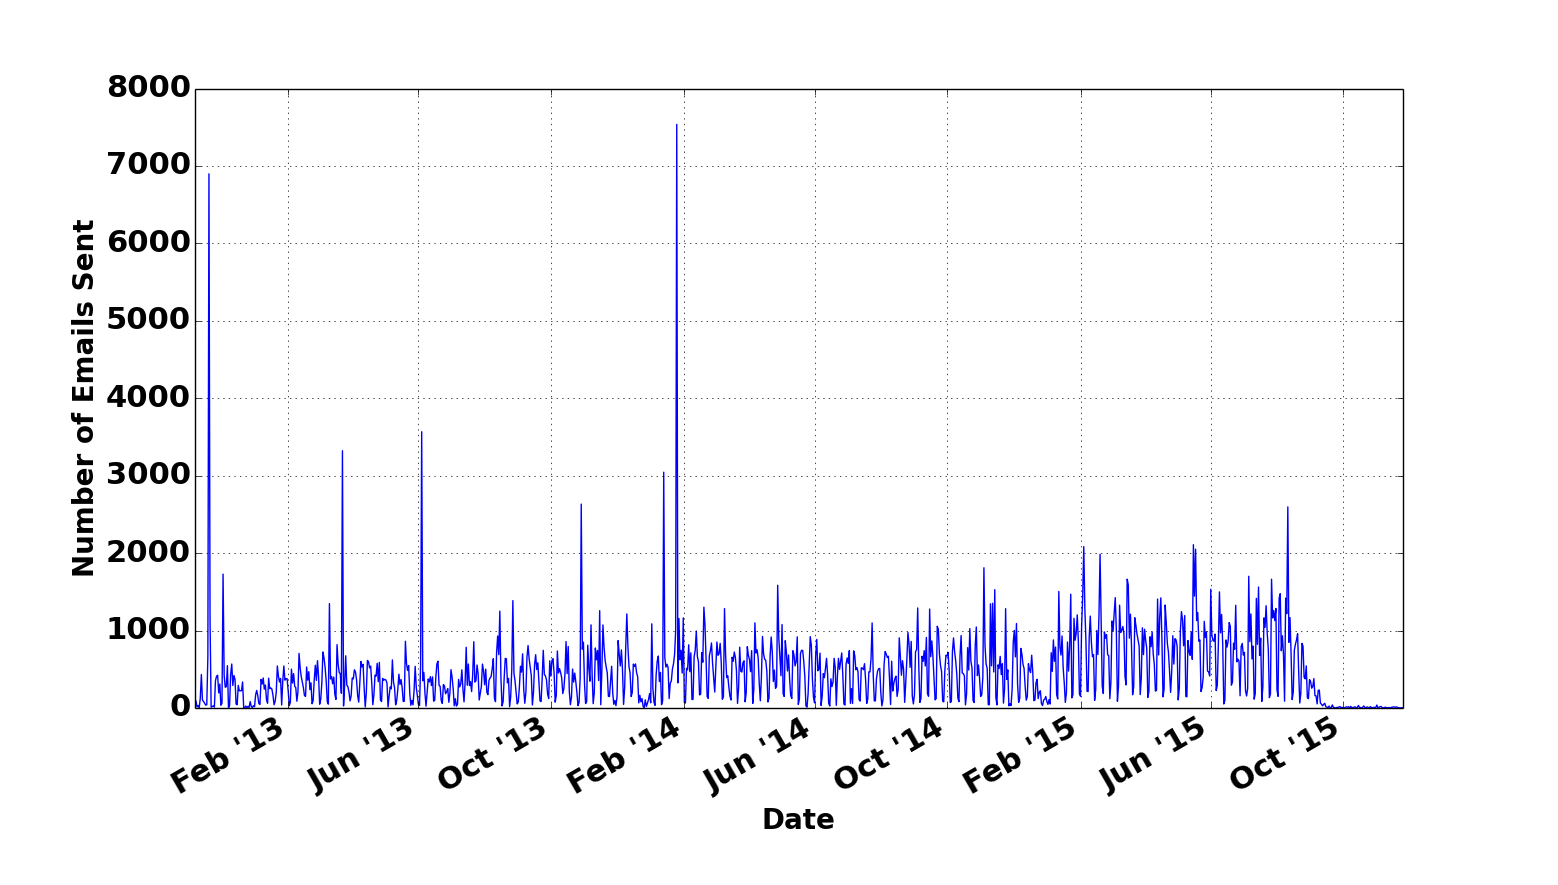
\includegraphics[width=\columnwidth,trim={0mm 0mm 0mm 0mm},clip]{emails_over_time}
	\caption[Center emails over time]{Number of emails sent in the database over time.  The data trends upwards as the center has grown.}
	\label{fig:emails_over_time}
\end{figure}


The center divides its employees into six main areas: directors, graduate students, operations, outreach, project management (PM), and research. 
Each person in the study was labeled with his or her job title.
One challenge of working with this dataset is that the distribution of these job titles is far from uniform.

A chart showing the distribution of employees into classes is shown in Figure \ref{fig:class_breakdown}.
Approximately half of the participants are graduate students, and there are only two outreach personnel included in the study.
Fig.~\ref{fig:db_bar} compares the distribution of job titles to the average number of emails per person per class.
Even though graduate students are by far the largest class, they send the fewest emails per person out of any class.
The directors exhibit opposite behavior: there are only eight directors in the center, but collectively their emails make up almost $50\%$ of the database.

\begin{figure}[t]
    \centering
        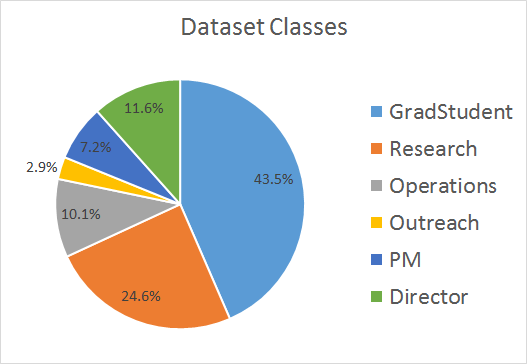
\includegraphics[width=\columnwidth,trim={0mm 0mm 0mm 0mm},clip]{class_breakdown}
        \caption[Dataset class distribution]{Pie chart showing the distribution of employee types in the dataset.  Note that the classes are far from being uniformly distributed.}
        \label{fig:class_breakdown}
\end{figure}


\begin{figure}[t]
	\centering
	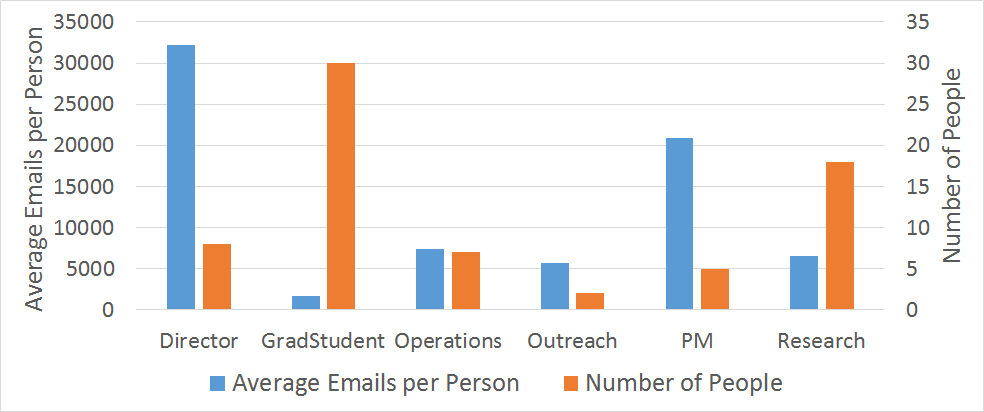
\includegraphics[width=\columnwidth,trim={2mm 2mm 2mm 2mm},clip]{DB_Stats_bar}
	\caption[Emails per person per job title]{Representation of each class in the dataset with respect to average emails per person and number of people.  Both distributions are very nonuniform, which poses a challenge to the classification algorithm.}
	\label{fig:db_bar}
\end{figure}


\section{Features} \label{sec:features}
The study uses 114 features that were extracted from the email data: 84 traffic-based and 30 social-based.
In the following sections, all features from each of the two categories are described. 
All of these statistics are used to characterize each employee of the center and serve as the inputs to the machine learning algorithm.
A full feature list is provided in Appendix B.

\subsection{Traffic-Based Features}
The traffic-based features are those calculated purely from the collected email metadata.
These metrics focus on the amount and types of emails each employee sends and receives.
This section details all of the traffic-based features used in this analysis and how they are calculated. 

\subsubsection{Email Counts and Email Types}
The simplest traffic-based features involve counting how many and what kinds of emails each participant sends and receives.
First, the total number of emails, total sent, and total received give a measure of how active an email user is on average.
These features can also indicate the direction tendencies of an employee's communication. 
Do they send more emails than they receive, or vice versa?  All of the traffic-based features detailed below consider direction.
Specifically, each metric is calculated three times: considering only sent emails, only received emails, and both sent and received emails.

Some traffic-based features focus on the different types of emails.
Two examples of these types of features are the number of emails sent directly to each employee and the number of emails where they were copied on the email.
The opposite direction of this was inspected as well, that is, the number of emails the employees sent directly to others and the number of copies sent out.
The average number of recipients on emails sent and received for each participant were also calculated.
Similarly, the number of emails sent and received as replies or forwards were used.
These measures give a sense of how the employee communicates with others in the organization and their connectedness.

Several features were calculated from just the subset of emails that were digitally signed.  These features were the total number of emails sent and received, number of unique email addresses, and the number of unique subjects.
These same metrics were also calculated for encrypted emails.

\subsubsection{Metadata Statistics}
The metadata of the emails contains extremely useful information.  This includes the email addresses involved, time stamp, the subject and body hashes and character counts, and the presence of any attachments.
From the time stamp, the time of day for each email was available.
The total number of emails with timestamps after hours were used as a metric.
For this purpose, after hours was defined as between 6pm and 7am EST on weekdays or anytime on weekends.
The timestamps were also used to calculate the average number of emails per day for each employee.
The mean and variance of the number of characters in the subject and body were calculated.
The total number of attachments sent and received were computed as well as the average number of attachments per email.

Some of the most interesting information came from email addresses and subject hashes of the emails.
The number of unique email address connections, both sent and received, was used as a feature.
By counting the number of identical hashed subjects, it was determined how many unique subjects were both sent and received from each employee.
The motivation behind these features is that employees with particular job titles may be more likely to be associated with long email chains, which would have the same subject.
It was hypothesized that staff members had more external communications than graduate students.
To test this, the number of emails sent and received from within the center and the university were calculated.
Email addresses with a Virginia Tech domain were considered to be affiliated with the university.
Email addresses with accounts on the internal mail server were labeled to be within the center.
Note that all employee email addresses of the center have a Virginia Tech domain, and are therefore also considered to be part of the university.


Most of the features described above involved raw email counts.
However, this could skew data by giving more importance to employees who have been associated with the center longer.
In order to normalize these values, corresponding percentage values were also fed into the learning algorithm.
Examples include the percentage of  sent emails that were sent after hours and the percentage of received emails with unique subjects out of all received emails.



\subsubsection{Most Useful Traffic-Based Features}
The best traffic-based feature for predicting employee status was the number of unique subjects received.
The metric used to evaluate features is mutual information.
This was used because it is integral to the machine learning algorithm as described in Section~\ref{sec:InfoGain}; details on the mutual information are provided in that section.
This number of unique subjects received represents how many distinct conversations involve each individual.
It is intuitive that people who are involved in more conversations hold a higher position in an organization because their input is requested more often.
A histogram showing the different values for this metric over the different job classes is shown in Figure~\ref{fig:traffic_ex_hist}.
This figure demonstrates how difficult this classification problem can be.
It is clear from the figure that graduate students participated in far fewer email conversations than any other group.
However, at least one graduate student is in six out of the first seven bins.
Another issue is that there are different personalities among the staff, which might explain why there are at least two research employees and at least one director in the first bin ($<500$) and last bin ($>5000$).
The divisions among the classes become slightly more clear when the feature values are normalized between 0 and 1, as opposed to the raw numbers shown here.
All feature values are normalized before being used by the learning algorithm.
\begin{figure}[t]
    \centering
        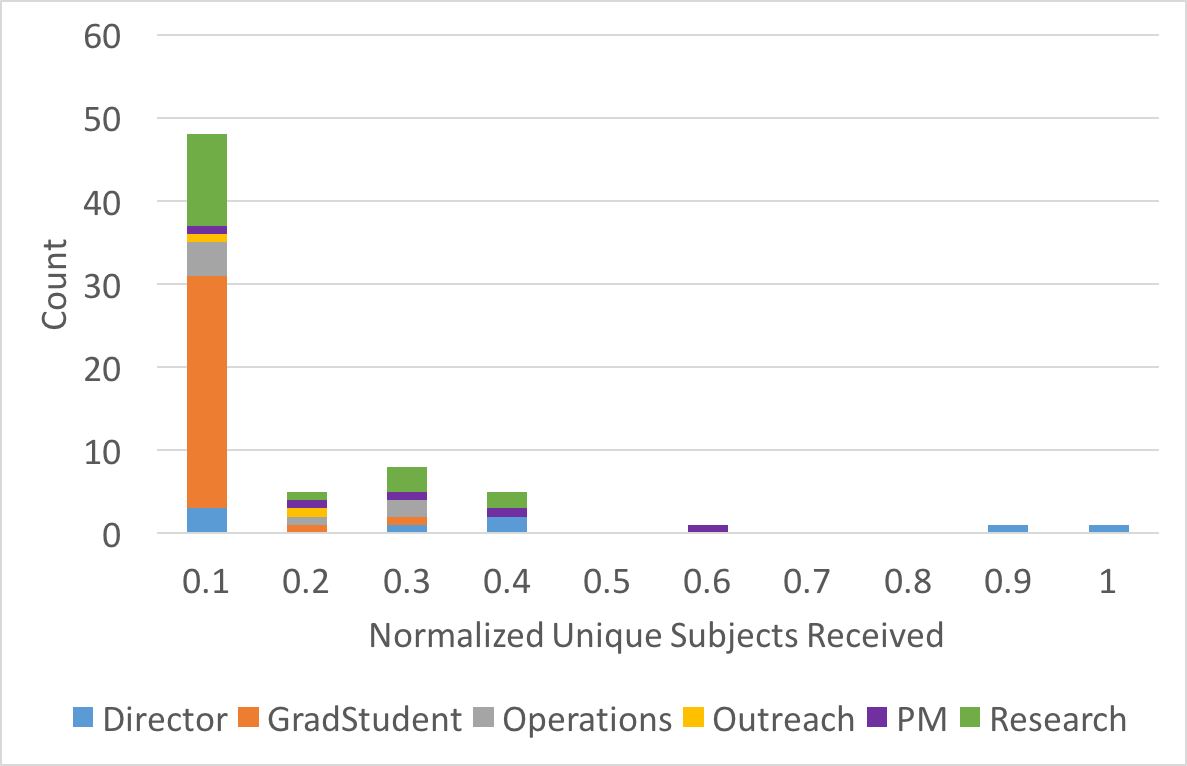
\includegraphics[width=\columnwidth,trim={0mm 0mm 0mm 0mm},clip]{Unique_subjects_rec_hist}
        \caption[Unique subjects received histogram]{Histogram of unique subjects received by job title.  Note that by using different thresholds, meaningful splits in the data can be made.  For example, employees with fewer than $500$ unique subjects received are likely to be graduate students, and employees with greater than $4500$ are likely to be higher status employees (i.e., Directors, PMs, some Research).}
        \label{fig:traffic_ex_hist}
\end{figure}

The second best traffic feature was the number of signed emails received.
Signed emails usually signal sensitive information.
Only certain groups within the center deal with this type of information, therefore it is understandable that this feature could help divide the subjects by title.
Finally, the third best traffic feature was the number of emails received as forwards.
Typically, those higher in the chain of command are forwarded emails where graduate students and lower-level employees are more likely to receive either replies or emails sent directly to them.
Notice that there are intuitive explanations behind all of the features selected by the ranker.


\subsection{Social Network Features}
In addition to tracking metadata statistics, features are also derived from modeling the emails as a social network.
The social features first transform email patterns in a graphical network and then calculate statistics from this model.


\subsubsection{Social Network Representation}
A social network is composed of nodes, which represent people, and edges, which represent the emails between people.
For this analysis, two different graphs were generated for analysis.
In the full graph, an edge exists between any two individuals that exchanged at least one email.
Each edge was given a weight equal to the total number of emails exchanged between the two employees.
The edges are undirected for this analysis.
A second graph only produces the same weighted edge between two nodes but only if at least 10 emails were exchanged.
The purpose of this second graph is to filter out stray single-email relationships between coworkers that do not constitute meaningful communication.
The full graph including all of the center employees is shown in Figure~\ref{fig:social_net}.  Note that graduate students are found on the fringes of the network and are generally the least connected.  However, there is a clear core group of employees that communicate very frequently.


\begin{figure}[t]
    \centering
    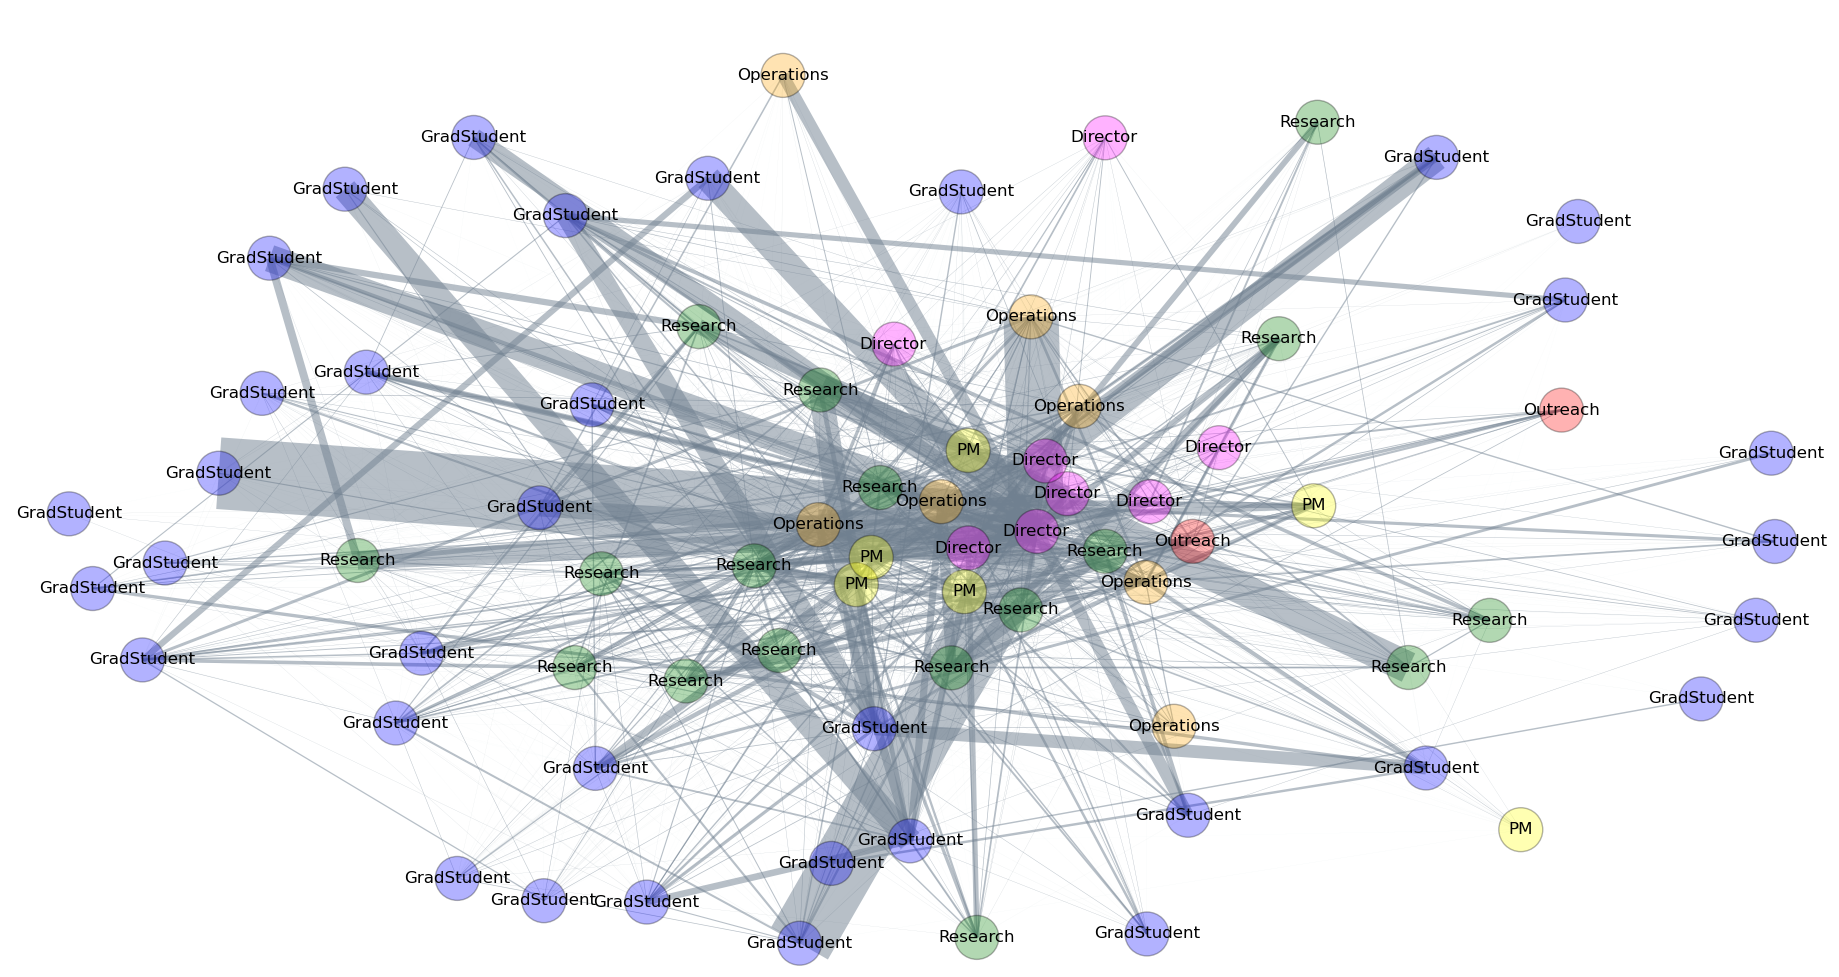
\includegraphics[width=\columnwidth,trim={0mm 0mm 0mm 0mm},clip]{color_social_network}
    \vspace{-17pt}
    \caption[The social network of the center]{A social graph representation of the center.  Nodes represent employees, and the thickness of the edges between nodes represent how many emails were exchanged.}
    \label{fig:social_net}
\end{figure}

Another representation of the full graph is shown as an adjacency matrix in Figure~\ref{fig:adj_matrix}.
Each of the two axes represent the employees of the center.
The color at each coordinate indicates how much communication existed between the two employees.
Some employees never exchanged any emails, while others exchanged many.

\begin{figure}[t]
    \centering
    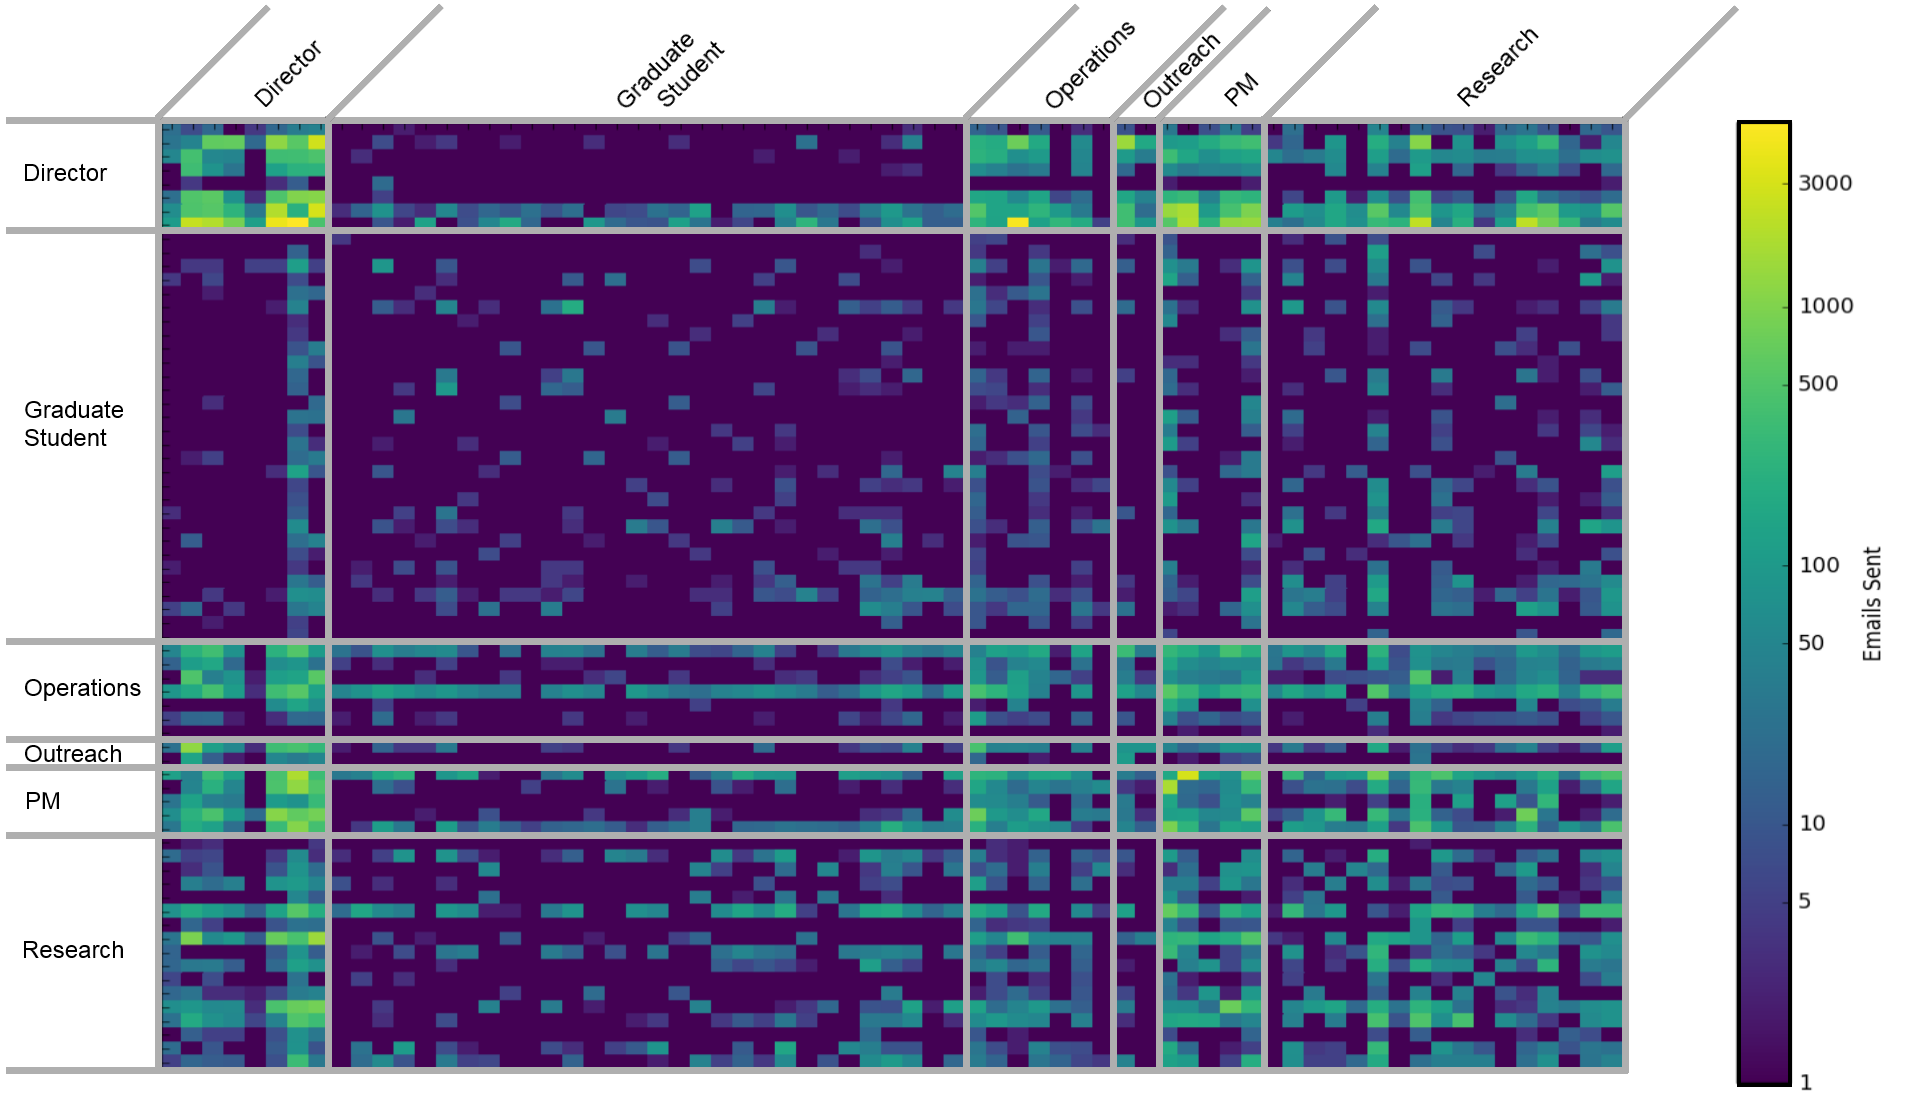
\includegraphics[width=1.05\columnwidth,trim={0mm 0mm 0mm 5mm},clip]{ViridisEdit}
    \vspace{-17pt}
    \caption[The dataset represented as an adjacency matrix]{The adjacency matrix representing the social connections of the center.  This graph overall is well connected and has just one component.  Nonetheless, there are many pairs of individuals who never exchanged a single email.}
    \label{fig:adj_matrix}
\end{figure}

Using this model, a suite of statistics can be calculated about the people in the graph.  The graphs were modeled in python.  The graph library networkx \cite{hagberg-2008-exploring} was used to calculate all graph features.

\subsubsection{Degree Measures}
The degree of each node, from both the full and partial graph, was used as a feature.  
The degree of a node $i$ is simply the number of other edges connected to node $i$.
All graph features were calculated once for the full graph and again for the partial graph.
The average neighbor degree was used as another feature.
The neighborhood of node $i$ is comprised of all nodes that are connected to $i$ via edges.
Therefore for node $i$, this metric averages the degree of each node in the neighborhood of $i$.
Mathematically, this is:
\begin{equation}
k_{\text{avg},i} = \frac{1}{|N(i)|}\sum_{j \in N(i)}k_j
\end{equation}
where $N(i)$ are the neighbors of node $i$ and $k_j$ is the degree of node $j$.
The distance between nodes was also used to generate some features.
In graph theory, distance is measured by the length of the path between two nodes.
Between node $i$ and any other node $j$ in graph $\mathcal{G}$, there exists a shortest path, $d(i,j)$.
The average shortest path between node $i$ and all other nodes in the graph, $d_{avg,i}$, was used as a feature.
That is,
\begin{equation}
d_{avg,i} = \frac{1}{n-1}\sum_{j \in \mathcal{V}, j\neq i}d(i,j)
\end{equation}
where $n$ is the number of nodes in graph $\mathcal{G}$ and $\mathcal{V}$ is the set of nodes in $\mathcal{G}$.
Similarly, the maximum shortest path length, or eccentricity, was used as a feature in the learning algorithm.
All of these measures can be interpreted to represent the centrality of a node.
If a node has many neighbors with large degrees or if it has very short maximum shortest paths it is probably representative of a person well-connected within the center.

\subsubsection{Cliques}
Some of the social features were based on existing graph theory concepts and algorithms.
For example, cliques.
If a subgraph of a graph $\mathcal{G}$ is maximally connected, that is all nodes are connected directly to each other, then this is called a maximal clique.
The number of cliques to which a node belongs was used as a feature.
The motivation behind using this metric is that it should mirror working groups within the center.
Therefore, the more groups an employee belongs to or communicates with, the more important they are assumed to be.

\subsubsection{Adapting Search Engine Algorithms}

The hubs and authorities of each node in both graphs were calculated.
The terms hubs and authorities come from the Hyperlink-Induced Topic Search (HITS algorithm)~\cite{kleinberg_hubs_1999}.
This algorithm was originally designed to rate web pages, but has since been applied to social networks.
A node's authority is just that\textemdash{}a measure of its importance over other nodes.
A node's hub score is a measure of how well-connected it is to other nodes.

Another algorithm used to generate features was the pagerank algorithm~\cite{page_pagerank_1999}, developed by Google to rank webpages for search results.
The assumption is that the most important webpages will be linked to frequently by other pages.
Therefore, the ranking is determined by estimating the quality and quantity of links to a node.
Both of these algorithms have been shown to predict expertise within an online social network~\cite{zhang_expertise_2007}.

\subsubsection{Clustering Metrics}
The triangle clustering coefficient~\cite{saramaki_generalizations_2007} was also used as a metric.
Consider a node $i$ with neighbors $m$ and $n$.
The triangle clustering coefficient, $C_3$,  measures the probability that $m$ and $n$ are also connected.
This is calculated by comparing the number of triangles within the graph to the maximum number of possible triangles in the graph.  If node $i$ has degree $k_i$, there can be at most $\frac{k_i(k_i-1)}{2}$ triangles formed in this subgraph.  Recall that the social networks are weighted graphs.  The weights of the graph are incorporated into this metric by finding the geometric mean~\cite{zhang_expertise_2007}.   Therefore, triangle clustering coefficient for node $i$, $C_{3,i}$, is:
\begin{equation}
C_{3,i} = \frac{2}{k_i(k_i-1)}\sum_{m,n}(\tilde{w}_{i,m}\tilde{w}_{m,n}\tilde{w}_{n,i})^\frac{1}{3}
\end{equation}
The edge weights in this calculation must be normalized compared to the maximum weight in the subgraph, i.e. $\tilde{w}_{i,m} = \frac{w_{i,m}}{max(w_{i,m})}$.

The square clustering coefficient~\cite{lind_cycles_2005} is very similar and was also used in the algorithm.
This metric, $C_4$, measures the probability that $m$ and $n$ are also neighbors to a fourth node, $p$.
This configuration would form a square.
To simplify the calculations, the graph for this metric is viewed without edge weights.
Therefore, the square clustering coefficient for node $i$, $C_{4,i}$, is the proportion of actual squares within a subgraph centered around node $i$ to the maximum number of possible squares in the same subgraph.
This is calculated as:
\begin{equation}
C_{4,i} = \frac{\sum_{m=1}^{k_i}\sum_{n=m+1}^{k_i}q_i(m,n)}{\sum_{m=1}^{k_i} \sum_{n=m+1}^{k_i}\left[a_i(m,n)+q_i(m,n) \right]}
\end{equation}
where $q_i(m,n)$ is the number of neighbors shared by $m$ and $n$, excluding $i$ and 
\begin{equation}
a_i(m,n) = (k_m-\eta_i(m,n))(k_n-\eta_i(m_n)) 
\end{equation}
where $\eta_i(m,n) = 1+q_i(m,n)+\theta_{mn}$.  
The indicator function $\theta_{mn}$ takes on a value of 1 if $m$ and $n$ are neighbors and equals 0 otherwise.
In theory, the higher the clustering coefficient, the more connected the node is within its neighborhood.

\subsubsection{Centrality Measures}
The majority of the social-based features were variations on centrality measures.
First is closeness centrality.
Closeness centrality, $C(i)$, is the normalized inverse of the sum of shortest path distances from node $i$ to all other nodes in the graph~\cite{freeman_centrality_1978}.  It is calculated as follows:
\begin{equation}
C(i) = \left(\frac{\sum_{j=1}^{n-1}d(i,j)}{n-1}\right)^{-1}
\end{equation}
where $n$ is the number of nodes in graph $\mathcal{G}$ and $d(i,j)$ is the minimum shortest path distance between node $i$ and node $j$.
Since for this application $\mathcal{G}$ is a weighted graph, shortest path distances are calculated using Dijkstra's algorithm~\cite{dijkstra1959note}.
This is true for all of the following algorithms that consider shortest path.

Next is betweenness centrality.
In a graph, there exists a shortest path between any node $s$ and any other node $t$.  Betweenness centrality of a node $i$, $C_B(i)$, is the sum of the percentage of all shortest paths in graph $\mathcal{G}$ that traverse node $i$~\cite{freeman_set_1977}.
It is calculated as:
\begin{equation}
C_B(i) = \sum_{s,t\in \mathcal{V}}\frac{\sigma(s,t|i)}{\sigma(s,t)}
\end{equation}
where $\mathcal{V}$ is the set of all nodes in $\mathcal{G}$, $\sigma(s,t)$ is the number of shortest paths between $s$ and $t$, and $\sigma(s,t|i)$ is the number of those paths that pass through $i$.
It is further defined that if $s=t$, then $\sigma(s,t)=1$ and if $i\in s,t$, then $\sigma(s,t|i) = 0$.

Degree centrality of a node $i$, $C_{d,i}$ is simply the percentage of nodes within the graph that are connected to node $i$~\cite{borgatti2011analyzing}:
\begin{equation}
C_{d,i} = \frac{k_i}{(n-1)}
\end{equation}
where $k_i$ is the degree of node $i$ and $n$ is the number of nodes in graph $\mathcal{G}$.

Current flow closeness centrality, also known as information centrality, is measured for each node.
In general, metrics related to current flow centrality differ from the previous centrality measures in that they consider all paths between nodes instead of exclusively shortest paths.
Current flow closeness centrality in particular was modeled after how current flows in electrical networks~\cite{brandes2005centrality}.
In circuits, current is distributed over the possible paths; in this metric a similar approach is taken to determine the information content of each path between two nodes.
For a graph $\mathcal{G}$ where all nodes are reachable, it is possible to construct a matrix $\boldsymbol{B}$ such that:
\begin{gather}
b_{ii} = 1 + \text{sum of weights of all edges connected to node } i \\
b_{ij} = 1- w_{ij}
\end{gather}
where $w_{ij}$ is the weight of the edge connecting nodes $i$ and $j$.
If $i$ and $j$ are not neighbors, $w_{ij}$ is defined to be $0$.
Denote $\boldsymbol{B}^{-1} = \boldsymbol{C}$.
From this matrix, the current flow closeness centrality of node $i$, $I_i$, is calculated as:
\begin{equation}
I_i = \frac{n}{nc_{ii}+T-2R}
\end{equation}
where $n$ is the number of nodes in $\mathcal{G}$; $T$ is the sum of the diagonal elements, $T = \sum_{j=1}^nc_{jj}$; and $R$ is the sum of any row in $\boldsymbol{C}$, $R = \sum_{j=1}^nc_{ij}$.
Note that because of the way it is constructed, each row in $\boldsymbol{B}$ will have the same sum.
This sum is equal to the number of columns in matrix $\boldsymbol{B}$, which is equivalent to the number of nodes in graph $\mathcal{G}$, $|\mathcal{V}|$.
A property of matrices states that if there exists a matrix where rows all add to the same value, $\lambda$, then all rows of the inverse of that matrix will sum to $1/\lambda$.
Therefore all rows of $\boldsymbol{C}$ will sum to $1/|\mathcal{V}|$, and $R$ is a constant that is not dependent on $i$~\cite{stephenson1989rethinking}.

Current flow betweenness centrality, as indicated by the name, also considers all possible paths between the source and target nodes.
This measure is also known as random walk betweenness centrality.
That is because it represents the expected number of times a random walk will cross node ${i}$ when it begins at node ${s}$ and ends at node ${t}$.
This is calculated as:
\begin{equation}
b_i = \sum_{i\neq s\neq t} r_{st}
\end{equation}
where $r_{st}$ is the element of matrix $\boldsymbol{R}$ which represents the probability that a random walk from $s$ to $t$ passes through $i$.

Another feature used by the algorithm is communicability centrality, or subgraph centrality~\cite{Estrada_2005}.  
To calculate this measure, consider all of the closed walks in graph $\mathcal{G}$, of length $k$.
Of those walks, those that begin on node $i$ are denoted as $\mu_k$.
A closed walk is any walk that begins and ends on the same node.
Repetition of either the edges and vertices is allowed.
The communicability centrality of node $i$, $SC(i)$ is computed as:
\begin{equation}
SC(i) = \sum_{k=1}^\infty \frac{\mu_k(i)}{k!}
\end{equation}

The final social network-based feature is 
communicability betweenness centrality.
This metric combines the concepts of current flow betweenness centrality and communicability centrality~\cite{estrada2008communicability}.
To compute the communicability betweenness centrality, consider the graph $\mathcal{G}$  with adjacency matrix $\boldsymbol{A}$.
Now consider $\mathcal{G}(r)$ which is identical to $\mathcal{G}$ except with all edges connected to node $r$ removed.
The adjacency matrix of $\mathcal{G}(r)$ can be written as $\boldsymbol{A}+\boldsymbol{E}(r)$.
$\boldsymbol{E}(r)$ has zeros in all elements except for those in the row and column corresponding to node $r$.
The values in these elements are the negative weights of the removed edges, i.e. $\boldsymbol{E}(r)_{ri} = -A_{ri}$.
The communicability centrality for node $r$ is therefore:
\begin{equation}
\omega_r \propto \sum_{p}\sum_{q} \frac{\left(e^{\boldsymbol{A}} \right)_{pq} - \left(e^{\boldsymbol{A}+\boldsymbol{E}(r)} \right)_{pq}}{\left(e^{\boldsymbol{A}}\right)_{pq}}, p\neq q \neq r
\end{equation}
The normalizing constant is omitted for clarity.
Note that all metrics used in the learning algorithm were normalized to be between 0 and 1.


\subsubsection{Most Useful Social Network Features}
The feature that was ranked the most useful social-network based feature by the feature ranker in Chapter~\ref{ssec:feature_select} was hubs.
Recall that a node's hubs value is an estimate of how well a node is connected to authorities.
These scores are calculated in an iterative reinforcement algorithm.
In the original website ranking context, a hub is a site that links to many sites that are determined to be relevant or important.
This can be interpreted to mean that employees with a high hubs score more often communicate with many of the directors or other important employees within the center.
The histogram of hub values in the partial graph broken down by class is shown in Figure~\ref{fig:social_ex_hist}.
Note that in this figure, the log of the hubs value is presented for visual clarity.
This figure shows more class division than Figure~\ref{fig:traffic_ex_hist}, as graduate students are limited to only the first four bins.
It appears that the same types of employees that had high unique subjects received counts also have large full graph hubs counts, specifically most of the Directors and PMs.

\begin{figure}[t]
    \centering
        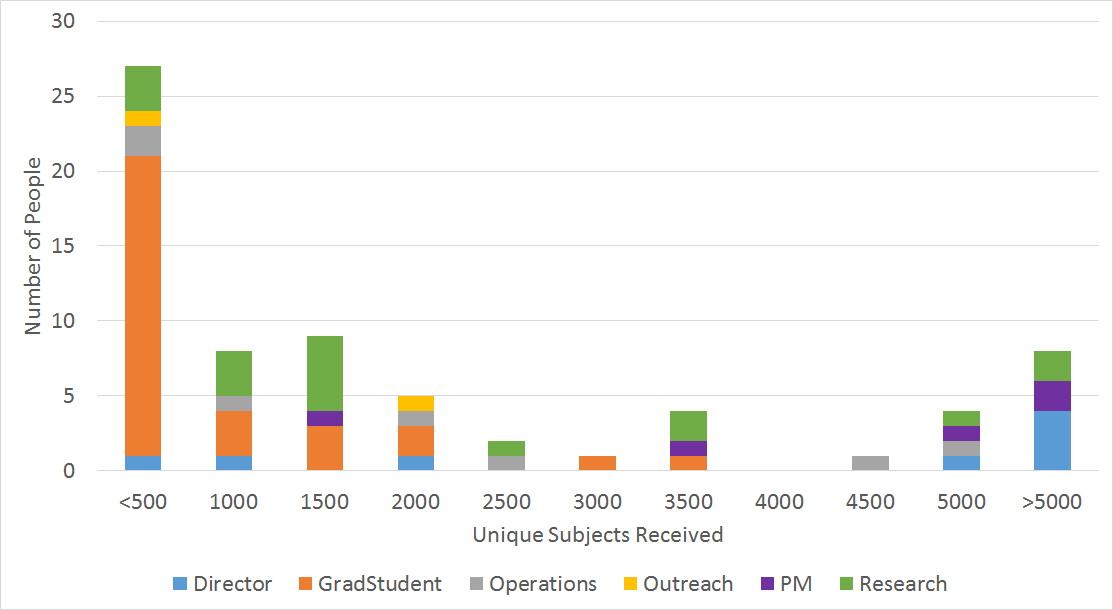
\includegraphics[width=\columnwidth,trim={2mm 3mm 2mm 3mm},clip]{Hubs_hist}
        \vspace{-17pt}
        \caption[Histogram of the hubs feature for the partial graph]{Histogram of hubs from the partial social graph by job title.  Note that directors on average have the highest hub score and graduate students have the lowest.  In fact, all graduate students have a full graph hubs score $<0.005$.  All but two PMs have a full graph hubs value $>0.025$.}
        \label{fig:social_ex_hist}
\end{figure}

The next two most useful measurements were the partial graph communicability centrality and the partial graph communicability betweenness centrality.
These measures may seem to have less intuitive interpretations than the top-ranked traffic-based features.
However, in general these centrality measures attempt to capture different aspects of how well a node is embedded within the graph.
In terms of this application, it measures how the breadth and depth of an employee's email communications within the center.

\chapter{Algorithm Design} \label{Algorithm}
This chapter describes the analysis behind the main algorithm: the random forest.
The first section describes the process of selecting the classification algorithm.
The second section discusses the theory behind random forests as well as the process of training and cross-validating the model.
The final section discusses the method behind ranking the different features used.

\section{Algorithm Selection}
Due to the large number of features and relatively low number of participants, a classification method was carefully chosen to avoid overfitting the data.
The first analysis that was performed was selecting an appropriate classification algorithm.
Considering only the 32 first-ring employees, those with less than 100 emails were removed.
The two outreach employees were also not included in this test.
The emails were randomly split with equal probability into training and testing sets.
Using these two sets of data, several different machine learning classification algorithms were evaluated using the java-based software package Weka~\cite{hall2009weka}.
The accuracy of each of these tests was recorded, and the best performers are shown in Figure~\ref{fig:algorithm_selection}.
The random forest algorithm was the most accurate.
This technique is popular in a variety of fields for being very robust to overfitting.
Furthermore, random forests were used in the work by Namata et al.~\cite{namata_inferring_2006}, which will serve as a benchmark for classification accuracy.

\begin{figure}[t]
	\centering
	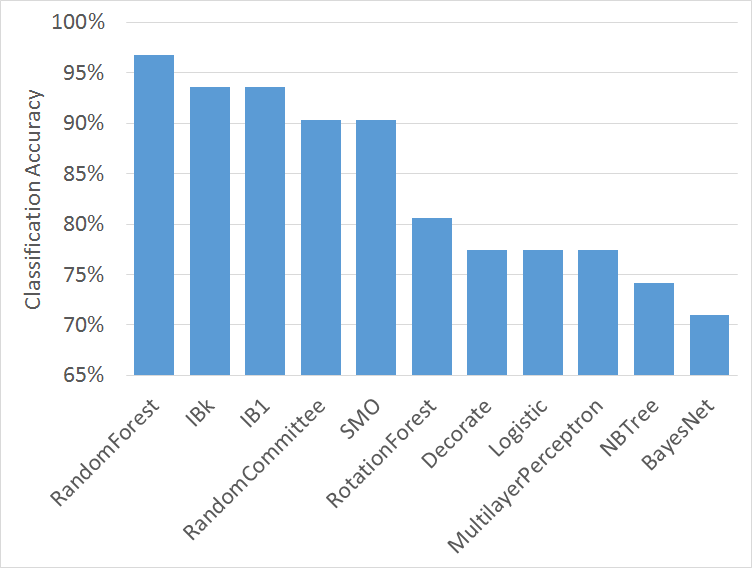
\includegraphics[width=0.8\columnwidth,trim={0mm 0mm 0mm 0mm},clip]{ModelSelection}
	\vspace{-12pt}
	\caption[Algorithm selection analysis]{Randomly generated training and test sets were used to evaluate several different classification algorithms.  Random forests were the most accurate and were therefore used for further analysis.}
	\label{fig:algorithm_selection}
\end{figure}


\section{Algorithm Description} \label{sec:InfoGain}
Random forests training is an ensemble method of machine learning comprised of many random trees.
While tree-based classifiers can be susceptible to overfitting, the random forest classifier has a lower variance and performs implicit feature selection to identify the most meaningful features.  
Weka uses the random forest based on the algorithm developed by Breiman~\cite{Breiman2001}.

A random tree is a machine learning algorithm that uses training data to divide and eventually label the data.
Each rule is designed such that it will split the data in a way that maximizes the mutual information.
These rules are constructed in a hierarchy that visually resembles a tree.
An example random tree with depth three is shown in Figure~\ref{fig:ex_tree}.

\begin{figure}[t]
    \centering
    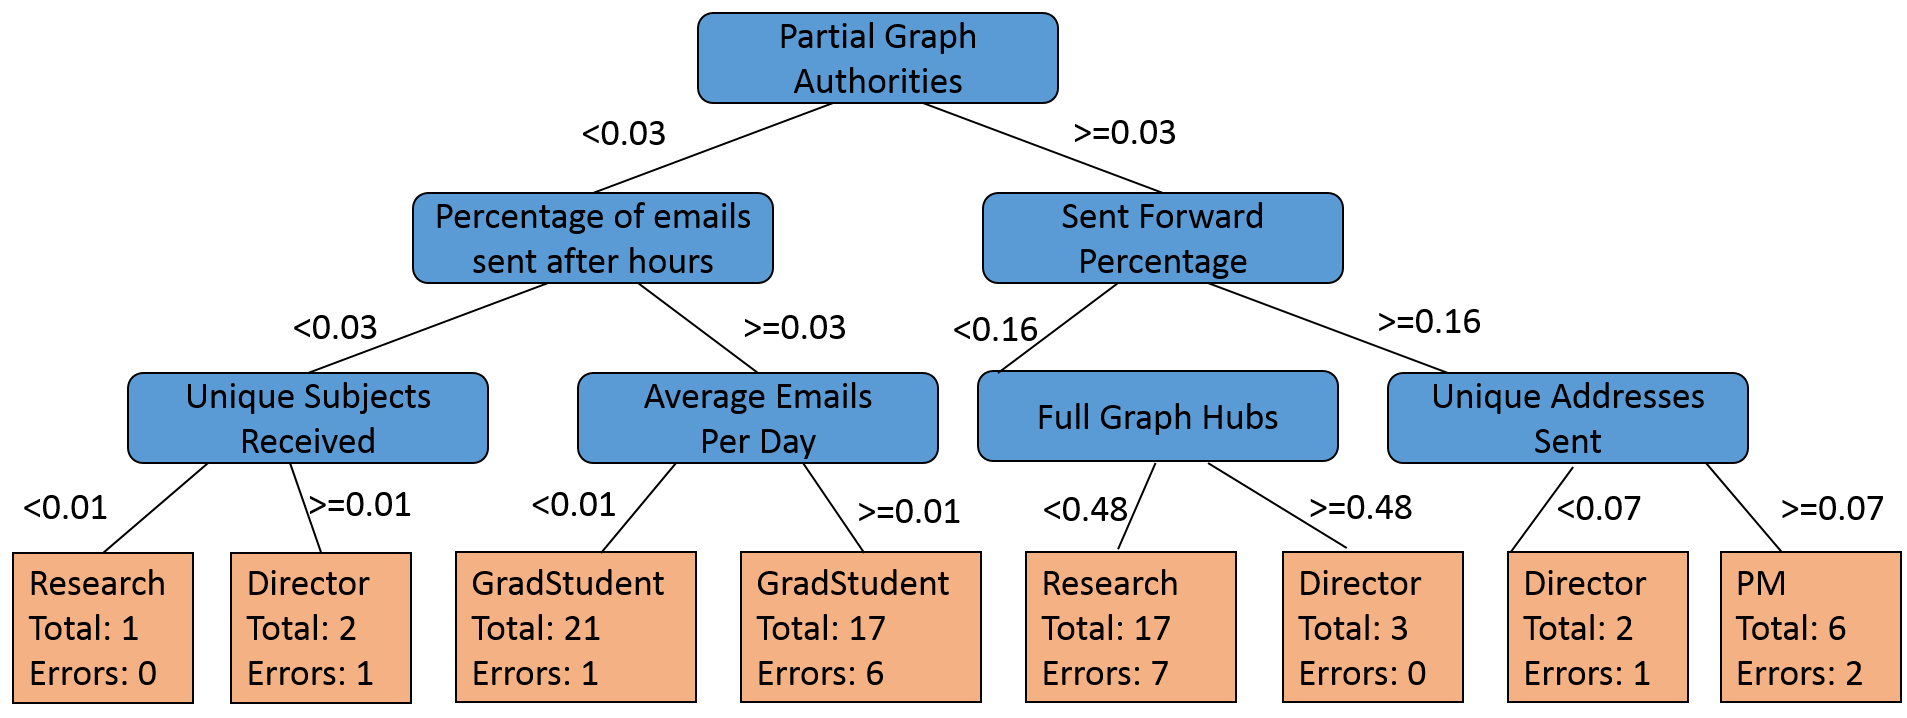
\includegraphics[width=\columnwidth,trim={0mm 0mm 0mm 0mm},clip]{3_level_tree}
    \vspace{-12pt}
    \caption[Example random tree]{Example random tree of depth 3 to demonstrate how a few rules can be used to find significant class divisions.}
    \label{fig:ex_tree}
\end{figure}

Random trees are built using a greedy heuristic that determines the best split at each level.
The best split is defined as the split which maximizes the mutual information and therefore makes the data after the split most homogeneous.
In this model, both the class and the features are treated as random variables.
The entropy of the class represents the amount of randomness in the class distribution, and is denoted as:
\begin{equation}
H(\text{Class})=\sum_{l\in \text{Labels}} p(l)\log p(l)
\end{equation}
The conditional entropy is evaluated for all available features.  
It represents the amount of randomness remaining in the class distribution when the attribute value is known.
The conditional entropy is calculated as:
\begin{align}
H(\text{Class}|\text{Attribute}) &= \sum_{a\in \text{Attributes}}p(a)H(\text{Class}|\text{Attribute}=a) \\
&=  -\sum_{a\in\text{Attributes}}p(a)\sum_{l\in\text{Labels}}p(l|a)\log p(l|a)
\end{align}
Mutual information represents how well knowledge of the attribute informs the prediction of the class.
Mutual information between the class distribution and the attribute is calculated as follows:
\begin{equation}
I(\text{Class}; \text{Attribute}) = H(\text{Class}) - H(\text{Class} | \text{Attribute})
\end{equation} \label{eq:info_gained}

The random tree algorithm splits on the attribute value that maximizes the mutual information.
Note that $H(\text{Class})$ is a constant, therefore the best attribute to split on, $A^*$, is:
\begin{align}
A^* &= \arg\max_a I(\text{Class}|\text{Attribute}) \\
&= \arg \max_a H(\text{Class})-H(\text{Class}|\text{Attribute})\\
&= \arg\min_a H(\text{Class}|\text{Attribute})
\end{align}

Note that the feature values used in this thesis are continuous, but the process above is described for discrete attribute values.
The feature values can be discretized by using thresholds instead.
If the feature values are sorting in ascending order, then a threshold can be defined between each consecutive pair of points.
These thresholds act as discrete ways to separate the data.
Therefore, the threshold that maximizes the mutual information, $T^*$ is:
\begin{align}
T^* &= \arg\min_t H(\text{Class}|\text{Threshold})\\
&= \arg\min_t H(\text{Class}|\text{Attribute}<t\})p(\text{Attribute}<t) \notag \\
 &\qquad \qquad + H(\text{Class}|\text{Attribute}\geq t)p(\text{Attribute}\geq t)
\end{align}

A visualization of the random forest training process is shown in Fig.~\ref{fig:rand_forest}.
Random forests build many deep random trees with imposed random variations.
Individually these random trees overfit the data.
To overcome this, these random trees are combined through a process of bootstrap aggregating, or bagging.
The bagging process involves each random tree generating a new training set by randomly sampling people from the input training set with replacement.
Each tree uses a different training set to build its rules.
For this analysis, each tree selects $\frac{2N}{3}$ samples to train the trees where $N$ is the number of data points in the overall training set.
Just as the samples were subsampled, so were the features.
Each tree can only use a small subset of the full feature set.
After all the trees are built, the test data is run through all the random trees in the forest.
Each tree outputs a prediction label for each data point, and the majority vote on each sample is the final predicted label.
In theory, the more meaningful features will drive some trees to make accurate predictions and will overrule trees that used the less informative features, effectively performing feature selection.
Random forest training reduces the variance and increases the accuracy of the model compared to a single random tree.

\begin{figure}[t]
	\centering
	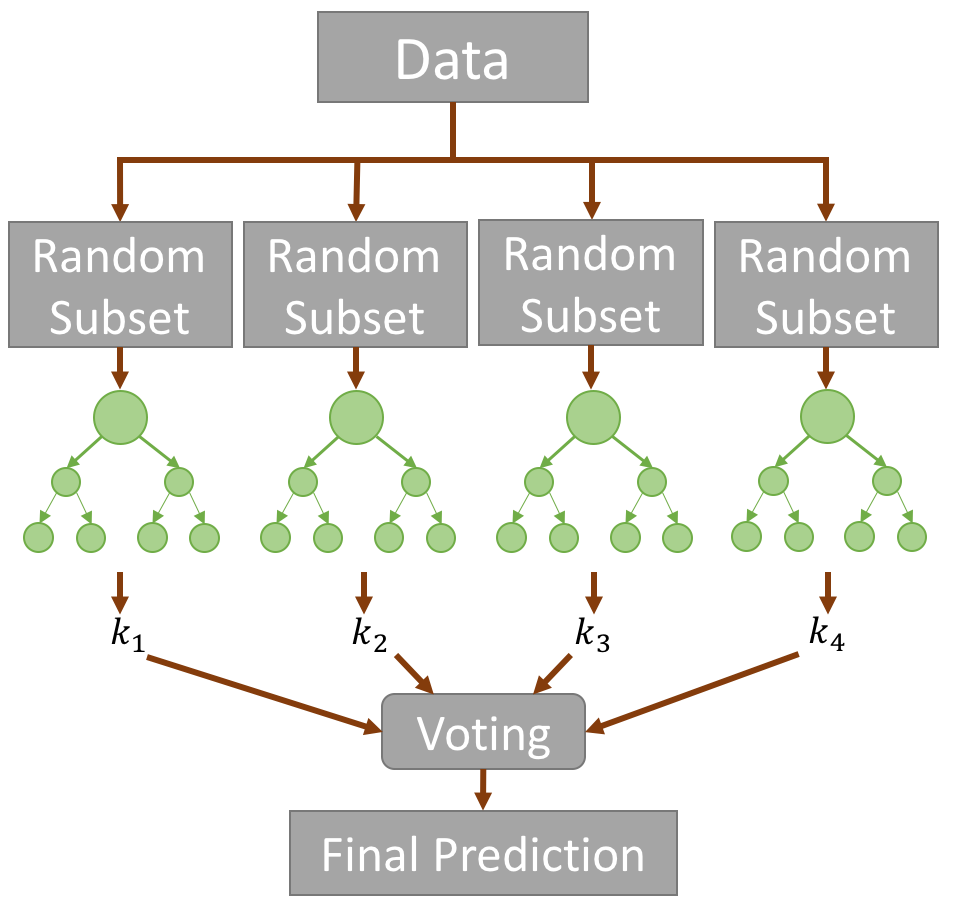
\includegraphics[width=0.6\columnwidth,trim={0mm 0mm 0mm 0mm},clip]{RandForest}
	\vspace{-15pt}
	\caption[Random forest prediction process]{A random forest builds many random trees using subsamples of the data.  Each tree generates a prediction for each test point, and the final prediction is decided by majority vote.}
	\label{fig:random_forest_diagram}
\end{figure}

To use this classification algorithm, the data must be split into three groups.
The emails in the dataset were randomly assigned to one of the following: 35\% for training, 30\% for validation, and 35\% for testing.
The training set was used to build the random trees.
The validation set was used in lieu of a test set to optimize the parameters of the random forest.
The testing set is used only once as the final evaluation of a model trained by the training set using these optimal parameters.

There are several parameters that were tuned to optimize this algorithm.
The first parameter that was analyzed was the percentage splits described above. 
Different sectioning percentages were tried for the training and validation sets, but 35\% for training and 30\% for validation produced the best validation accuracy.
This is likely because it is nearly an even split between the two sets.
From validation analysis, the optimum number of trees in the random forest was determined to be 750.
Another test found that each tree should subsample of 7 random features for maximum validation accuracy.
This value represents approximately 6\% of the total available features.



\section{Feature Selection} \label{ssec:feature_select}
Random forests can be difficult to interpret because the ensemble method obscures which features are most meaningful.
An attribute analysis helps to better understand which features are better label predictors.
Since random trees use mutual information to dictate splits, mutual information was used as the evaluation criteria for the features.
Each attribute was evaluated by measuring the mutual information with respect to the class, and each attribute was ranked in order of most important to least.
Table~\ref{tab:ranked_feats} shows the top twenty features from this analysis and the features' corresponding mutual information.  
Highlighted rows represent the features not used previously in email analysis.
Note that in this table, the features are almost perfectly split between the two types.
Nine of the features are traffic-based and eleven are social-based.
This highlights the importance of using both types of features in this analysis because both types of features contain valuable information related to the class of an individual.


\begin{table}[t]
\caption{Top 20 features ranked by the mutual information.}
\centering
\label{tab:ranked_feats}
\resizebox{0.75\columnwidth}{!}{%
\begin{tabular}{@{}lrr@{}}
\toprule
Feature                                      & Type         & Information Gain\\ \midrule
Partial graph hubs                           & Social        & 0.589  \\
Full graph hubs                              & Social        & 0.554  \\
Number of emails received as forwards        & Traffic      & 0.554  \\
\rowcolor{Gray}
Number of signed emails received             & Traffic      & 0.514  \\
\rowcolor{Gray}
Number of signed emails received with unique subjects & Traffic & 0.514\\ 
Partial graph current flow closeness centrality & Social    & 0.512  \\
Partial graph pagerank                       & Social       & 0.512  \\
Number of emails received as copies   & Traffic      & 0.500  \\
Number of emails received from center employees & Traffic	    & 0.492  \\
Full graph current flow closeness centrality & Social       & 0.492  \\
Full graph pagerank                          & Social       & 0.492  \\
Average number of emails received per day    & Traffic      & 0.489  \\
Partial graph communicability centrality     & Social       & 0.486  \\
\rowcolor{Gray}
Partial graph communicability betweenness centrality & Social & 0.486  \\
Average number of emails per day (both sent and received) & Traffic & 0.479    \\
Number of emails sent to center employees      & Traffic	    & 0.476  \\
Partial graph number of cliques              & Social       & 0.470  \\
Percentage of emails received as forwards    & Traffic      & 0.451  \\
Partial graph degree centrality				 & Social		& 0.448  \\
Partial graph average shortest paths         & Social	    & 0.448  \\ \bottomrule \\
\footnotesize Note: Highlighted rows represent features unique to this work.

\end{tabular}
}
\end{table}


\chapter{Performance Analysis} \label{Performance}
The first result shows the algorithm's ability to correctly classify both the study's volunteers and the peripheral employees identified from the volunteers' emails.
The second part of the results assumes perfect labeling of the employees and analyzes interactions between employees of different job titles.
The ultimate goal of this research was to determine what additional information can be gained by analyzing the organic organizational chart when compared with the official organizational chart.

\section{Classification Results} \label{ssec:classification_results}
As described in Section~\ref{sec:InfoGain}, data was split by randomly assigning each email to training or testing sets with equal probability, $0.35$.
The remaining 30\% of the data was used as a validation set.
Then, all of the metrics described in Section~\ref{sec:features} were calculated for both groups separately.
The training data was used as input to the random forest algorithm as described in Section~\ref{sec:InfoGain}, validation was performed, and predictions were generated for the test data.
The number of correct and incorrect classifications for each class are shown (below) in Figure~\ref{fig:result_hist}.
Note that only three predictions were wrong: two people in research were misclassified as graduate students and one graduate student was misclassified as research.
It is important to note that two out of the three misclassifications are peripheral employees.
Therefore, the classification accuracy for the study participants is 97.3\%, correctly classified peripheral employees is 93.8\%, and the overall accuracy of this method using all features is 95.7\%
The confusion matrix for this analysis is another way to visualize the results, as shown in Figure~\ref{fig:conf_matrix}.

\begin{figure}[t]
    \centering
    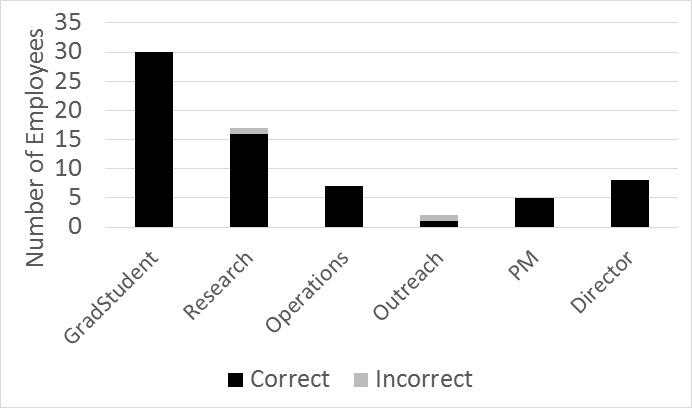
\includegraphics[width=\columnwidth,trim={0mm 0mm 0mm 0mm},clip]{Prediction_50_50_RF}
    \vspace{-20pt}
    \caption[Job title classification results]{The random forest algorithm was extremely accurate even for very uneven class sizes.  Note that all members of 4 classes were labeled perfectly.  There were only 2 errors out of 69 employees, both of which for employees who did not provide emails for the study.}
    \label{fig:result_hist}
\end{figure}


\begin{figure}[t]
    \centering
        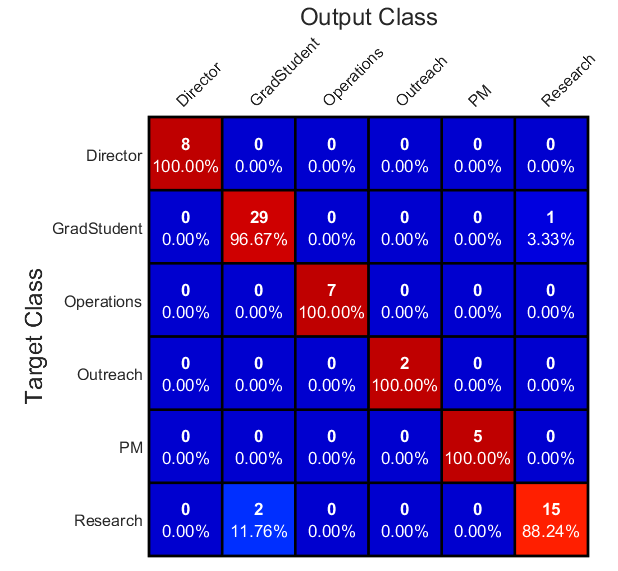
\includegraphics[width=.7\columnwidth,trim={0mm 0mm 0mm 0mm},clip]{Classification_confusion}
        \vspace{-7pt}
        \caption[Job title prediction confusion matrix]{Confusion matrix for the job prediction test.  The only two classes that confused the classifier were graduate student and research, making a total of 3 errors.  These classes are very similar, so it is understandable that there would be errors.}
        \label{fig:conf_matrix}
\end{figure}


On further inspection, the errors made by the learning algorithm can be explained by understanding center operations.
The distinction between graduate students and research faculty is likely the least clear for two primary reasons.
First, some PhD students have been at the center as long or longer than some research faculty.
This leads to older PhD students having larger email counts than some of the newer research staff, which could trick the algorithm.
Some research faculty are also students, which may cause their email communication patterns to more closely resemble graduate students. 
To further complicate matters, some graduate students joined the center as staff after they graduated.

Note that this method relies on some assumptions.
One is that employees with the same title exhibit similar email behavior.
Overall, based on the success of the algorithm and the distributions of the histograms, this seems to prove true.
Another premise underlying this analysis is that peoples' email behaviors are consistent over time.

An experiment was performed to evaluate this second assumption.
All employees with less than ten months of consistent email behavior were removed from this experiment.
Consistent email behavior was defined as sending or receiving at least one email per month.
One month of email data per person was set aside to act as a training set.
The random forest algorithm with the parameters described in Section~\ref{Algorithm} was trained using the first month's data.
Each of the nine subsequent months became a separate test set.
The features were calculated for each of these months, and the accuracy of the model on the test sets was calculated.
The result is a test that evaluates how the average email behavior of the center changes over time, as depicted in Figure~\ref{fig:time_analysis}.
As the figure shows, there is a decrease in algorithm performance as the time between the training data and the test data increases, but this decrease occurs at a slow rate.
Note that with six months separating the training data from the test data, the algorithm still performed with 63.4\% accuracy.
This is a decrease of less than 6\% from when the test data is from the month immediately following the training data.


\begin{figure}[t]
    \centering
        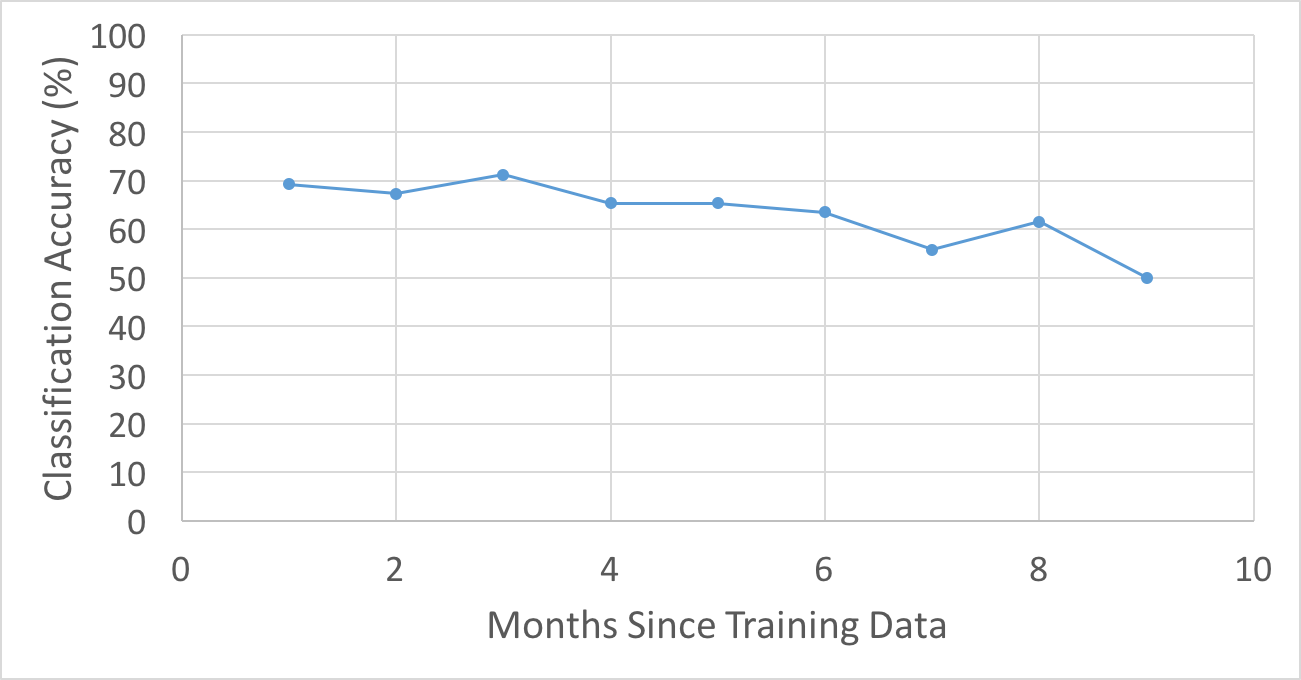
\includegraphics[width=.8\columnwidth,trim={0mm 0mm 0mm 0mm},clip]{TimeGapsAnalysis}
        \vspace{-7pt}
        \caption[Accuracy of classification over time]{As time between the training data and the testing data increases, the accuracy of the prediction algorithm slowly decreases.  This reinforces the assumption that the email behavior of the center employees is relatively constant in time.}
        \label{fig:time_analysis}
\end{figure}

To determine which features were necessary to the analysis, the algorithm was run several times with a subset of the features.
The first subset used only the top twenty features from Table~\ref{tab:ranked_feats}.
For each subsequent run, the least useful feature according to the feature analysis was removed from the input to the system until only one feature remained.
A plot of this analysis is shown (below) in Figure \ref{fig:feat_analysis}.
The maximum accuracy using twenty or fewer features was achieved when either the top fifteen or sixteen were used.
For this scenario, there were only 6 errors, resulting in 89.86\% accuracy.
This is only three more errors than was found using all 114 features.
Even using just the top two features resulted in classification accuracy over 86\%.
Therefore, a very good classifier can be built using much fewer features if the features are selected properly.

\begin{figure}[t]
    \centering
        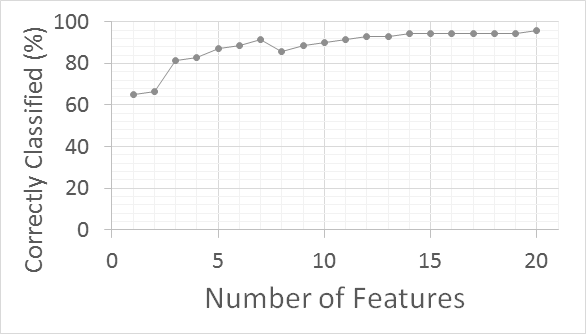
\includegraphics[width=.8\columnwidth,trim={0mm 0mm 0mm 0mm},clip]{FeatureAnalysis}
        \vspace{-7pt}
        \caption[Prediction accuracy compared to number of features]{Prediction accuracy compared to number of features used for analysis.  Note that the accuracy is still very high, 89.86\%, when only fifteen features are used.  The outcome of using only the top twenty features produces three classification errors, only one more than using the full set of 114 features. }
        \label{fig:feat_analysis}
\end{figure}

\section{Leave-One-Out Cross-Validation}
Leave-one-out cross-validation (LOOCV) was used as an alternative evaluation method because it removes the time-based assumption.
For LOOCV, all of the data is used to calculate the features.
Then, all but one person is used as training and the left-out person is used as a single test point.
For this experiment, the 2 people of the outreach class were removed because that would result in only one training point for that class.
By testing each point this way, it is possible to evaluate the classification algorithm without having data from all employees in both the training and test sets.
This method ensures that the algorithm is not learning each person's behaviors individually.
The results of this test are reported below in Figure~\ref{fig:loocv_conf_plot}.
\begin{figure}[t]
    \centering
        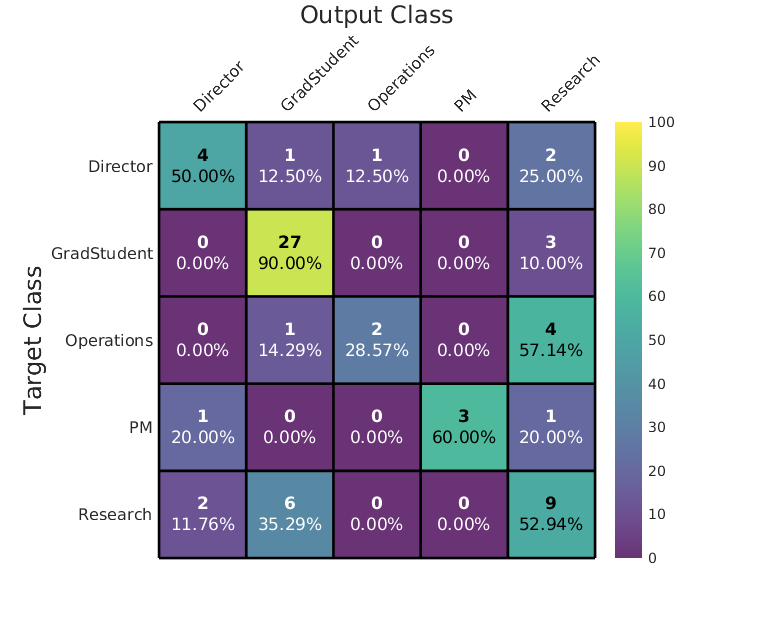
\includegraphics[width=.7\columnwidth,trim={0mm 0mm 0mm 0mm},clip]{LOOCV_confusion}
        \vspace{-7pt}
        \caption[Leave-one-out cross-validation results]{Prediction accuracy was higher for graduate students, who have more uniform behaviors and more training data.  However, for each category, the majority of the people classified were true members of that group, save for research.}
        \label{fig:loocv_conf_plot}
\end{figure}

This analysis resulted in a lower accuracy than the previous experiment.
In total, only 65.7\% were correct.
The category of graduate student was the easiest to predict and the operations class was the most difficult.
This result is understandable because the employees within operations perform the widest range of duties, including technical, administrative, and program support.
However, note that for each category the majority of the people classified were true members of each group, except for the research category.
Even out of those classified as research, there were more true researchers than any single other class.

Namata et al. performed the same analysis on the Enron email corpus~\cite{namata_inferring_2006}.
Compared to the dataset used in this analysis the Enron data involved many more people.
The Enron dataset has employees distributed more evenly into six classes, one more than used in the analysis above.
Even with these advantages, the previous work was only able to achieve 62.09\% LOOCV accuracy.
The difference between that analysis and the work described in this thesis is that Namata et al. only used traffic-based features.
This analysis shows that integrating social-based features with the traffic-based statistics can improve job classification results.

\section{Hierarchy Analysis}
The purpose of this hierarchy analysis was to compare the email relationships from the data with the official project groups of the center.
A combination of the predicted labels from Section~\ref{ssec:classification_results} and the email patterns from the data generated the organic hierarchy for the center, shown in Fig.~\ref{fig:generated_hierarchy}.
Although the center has a very flat structure, project information often flows from directors to project managers down to research staff and finally graduate students.
Outreach and operations personnel are not actively involved in project work, and are therefore omitted from this chart.
The nodes of the graph represent anonymized job titles for the employees of the center.
The output of the classification algorithm was used as the source of these job titles.
Note that in this figure, the employees with the incorrect classification labels are outlined in red.
Therefore, the two research staff are labeled as graduate students, and the mislabeled graduate student is given the title of research.
Edges are drawn for each layer based on how many emails were sent to each employee in the layer above.
For example, each graduate student has three edges corresponding to the three researchers they emailed most frequently.
The most emailed researcher is the darkest line, the second-most common researcher is more transparent, and the third-most common link is the most transparent.

\begin{figure}[t]
	\centering
	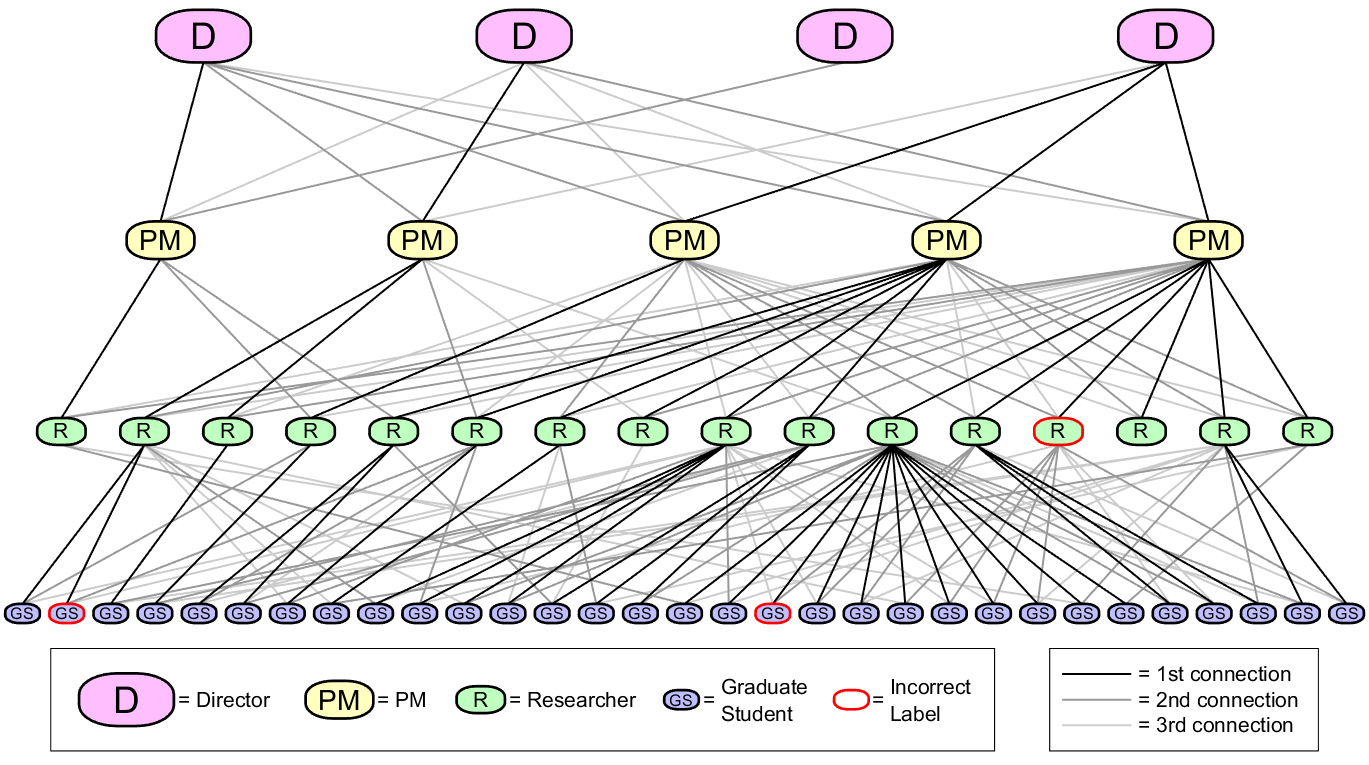
\includegraphics[width=1.05\columnwidth,trim={0mm 0mm 0mm 0mm},clip]{org_chart_with_legend}
	\vspace{-7pt}
	\caption[Generated organic organization chart of the center]{The generated organic organization chart of the center using the previous analyses.  This chart could be used as a tool in corporate reorganizations to analyze workload and coworker relationships.}
	\label{fig:generated_hierarchy}
\end{figure}

This type of chart could be used as a tool for understanding the underlying structure of a company in order to analyze possible reorganizations.
If the center was considering dividing into two offices, this chart could help identify clusters that signal the optimal partition.
Another feature of this graph is the disparity in project manager connections.
Perhaps the various PMs perform different functions; some communicate more closely with researchers than others.
It is also possible that some of the PMs with many researcher connections are overloaded, and the organization could benefit from redistributing projects.
The final interesting thing to note about this graph is that the researcher outlined in red is in fact a graduate student.
However, that person has three primary graduate student connections.
If this student were to graduate and be hired on as a research staff, this figure indicates which graduate students he or she could help mentor.
This organic organization chart reveals underlying relationships within the center.

To generate a measure of how well the email-based organic structure compares to the organizational chart, the relationships in Fig.~\ref{fig:generated_hierarchy} and the rest of the email data were compared to the official hierarchy.
Most of the employees at the center are organized under a director and many work with a program manager (unless for example they are a director or program manager).
Therefore, from knowledge of the center, employees were labeled with their official director, and research staff and graduate students were labeled with their primary program manager.
Note that these labels were not available for all participants in the study.
To generate a metric of how well emails can be used to predict the center's organizational chart, the director and project manager for each applicable employee is predicted from the email metadata. 
This analysis was broken down by class and plotted in Figure~\ref{fig:project_classify}.

\begin{figure}[t]
	\centering
	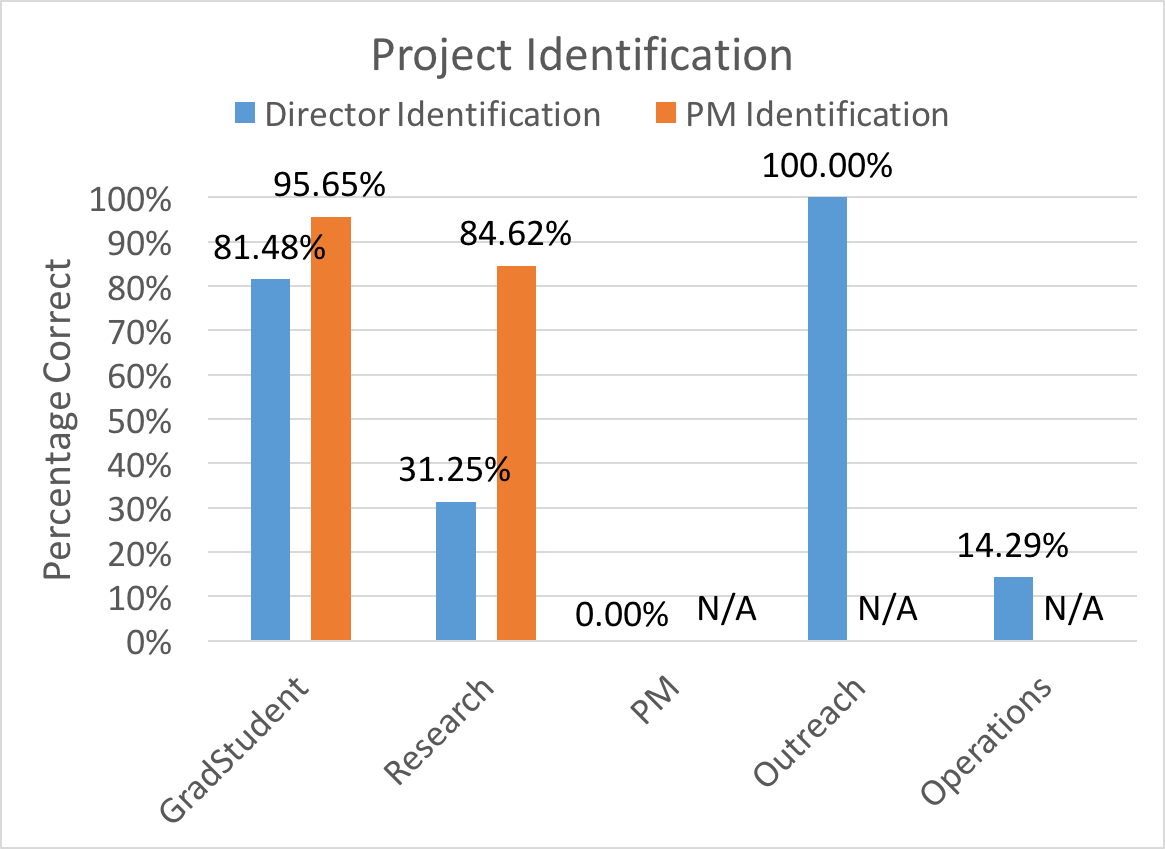
\includegraphics[width=0.8\columnwidth,trim={2mm 2mm 2mm 2mm},clip]{superior_identification}
	\vspace{-7pt}
	\caption[Project manager and director prediction results]{The accuracy of the director assignment appears to vary greatly between classes.  However, the assigned project manager of researchers and graduate students is accurately predicted from the email data.}
	\label{fig:project_classify}
\end{figure}


The director of each employee is predicted by the algorithm to be the director that the employee communicated with most by email.
Only 52.63\% of the center's employees communicate most frequently with their official director.
This result points to a possible disconnect between the official organization chart and the organic relationships within the center.

To identify each employee's project manager ground truth is selected to be the project that primarily funds the employee.
This time, 91.67\% of graduate students and researchers communicate most frequently with their primary program manager.
The relation between employees to project managers appears to be stronger than that with directors.
From knowledge of the center, it appears that the few errors in this classification are due to employees who work with multiple project managers.  

It appears that in general, graduate students are very likely to regularly email their assigned director and project manager.
Members of the research staff communicate predictably with their primary program manager, but the director relationships from the organization chart are not reflected in the email data.
Project management and operations also seem to exhibit a disconnect between the official director of each group and the directors they email.


\chapter{Future Work} \label{FutureWork}
There are obvious limitations with this dataset due to its small size.
It is also not clear how well these methods and results would generalize to other email datasets, however such datasets are not publicly available.
This chapter details what analyses could be possible given a larger dataset.
The first section of this chapter presents some analysis showing that more data would improve the classification performance.
The second section describes a deep learning method that could be used as a classifier if a massive dataset were available.
The third section considers possible paths forward with this work.
\section{Improving LOOCV Accuracy}
As discussed above, the accuracy of the leave-one-out cross-validation test was low because of the limited number of data points.
The confusion matrix in Figure~\ref{fig:loocv_conf_plot} shows that about one third of the predictions were incorrect.  
These results can typically be improved by increasing the amount of training data. 

An experiment was performed to gauge how the amount of training data affects the accuracy of the LOOCV test.
A series of eleven time periods were set for each person in the study, ranging from one week to ten months.
Only the 37 employees who sent or received at least one email per week for ten months were included in this analysis, which is a much smaller population to test than what was used in the LOOCV analysis in Ch~\ref{Performance}.
Some of these 37 employees were direct participants in the study, but the remaining .
For each employee's time slices, the features were calculated separately and then LOOCV was performed on each time slice.
For example, the first run considered the most recent week of email history for each person.
The LOOCV accuracy from only one week of data is obviously very low - approximately 32\%.
Then the test was run on the next time slice, which was the most recent two weeks.
This process was repeated until LOOCV was performed on 10 months of data for each person.
The results of this analysis are shown in Figure~\ref{fig:loocv_generalization}.
As the number of days of data increases, the accuracy increases slowly and the variance in the accuracy decreases.
A logarithmic curve fit to the data is shown.
This shows that more data, as measured by time, in general increases classification accuracy.
\begin{figure}[t]
    \centering
        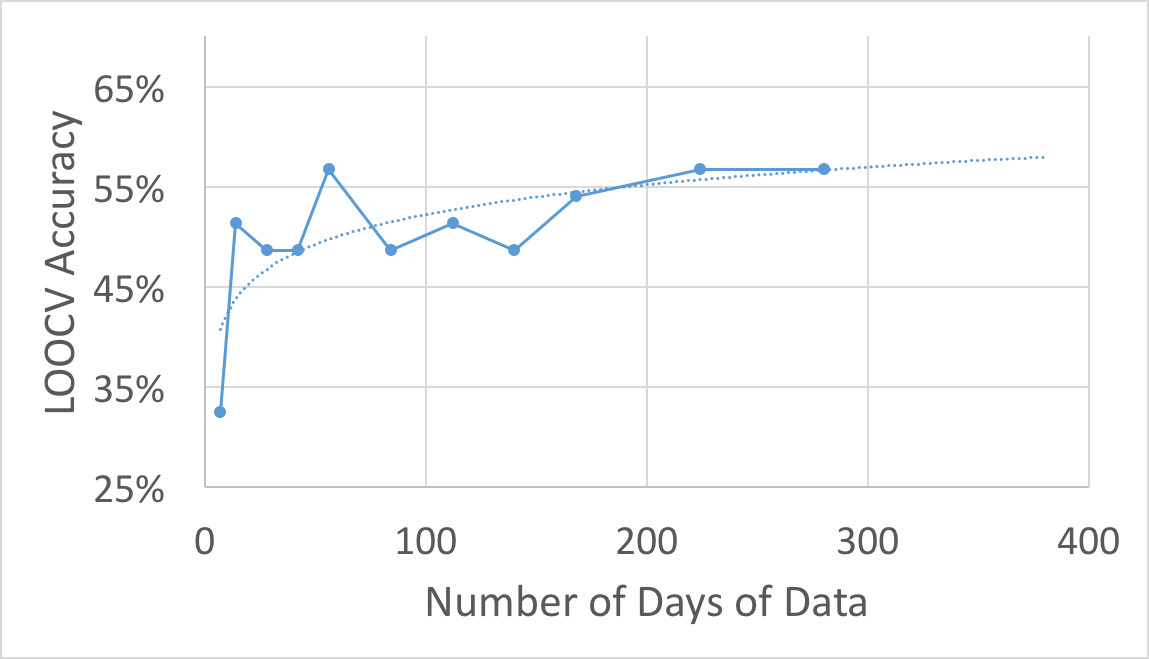
\includegraphics[width=.7\columnwidth,trim={0mm 0mm 0mm 0mm},clip]{num_days_LOOCV}
        \vspace{-7pt}
        \caption[Effects of more data on prediction accuracy]{Effects of using more data for leave-one-out cross-validation.  As the number of days of data increases, the accuracy increases slowly and the variance in the accuracy decreases.  This implies that more email data can increase classification accuracy.}
        \label{fig:loocv_generalization}
\end{figure}

The improvement with additional data shown in Figure~\ref{fig:loocv_generalization} is modest.
Recall that the size of the population under test was decreased because of the consistent behavior constraints.
In order to investigate the effect of more data, as measured in people, another test was performed.
Starting with the original 67 employees (removing the two outreach employees), a random five employees were removed from training data and the LOOCV accuracy was measured for the remaining 62.
To combat variance due to the randomness of removing employees, the test was repeated five times and the results averaged.
Then, ten random employees were removed from the original training data and test.
This continued until only seven employees remained.
These results are shown in Figure~\ref{fig:people_generalization}.
Similar trends are exhibited between this plot and the previous, namely decreasing variance and increasing accuracy.
Again, a logarithmic trendline is shown for reference.
It is clear that adding more people, in general, improves the performance of the classifier.
\begin{figure}[t]
    \centering
        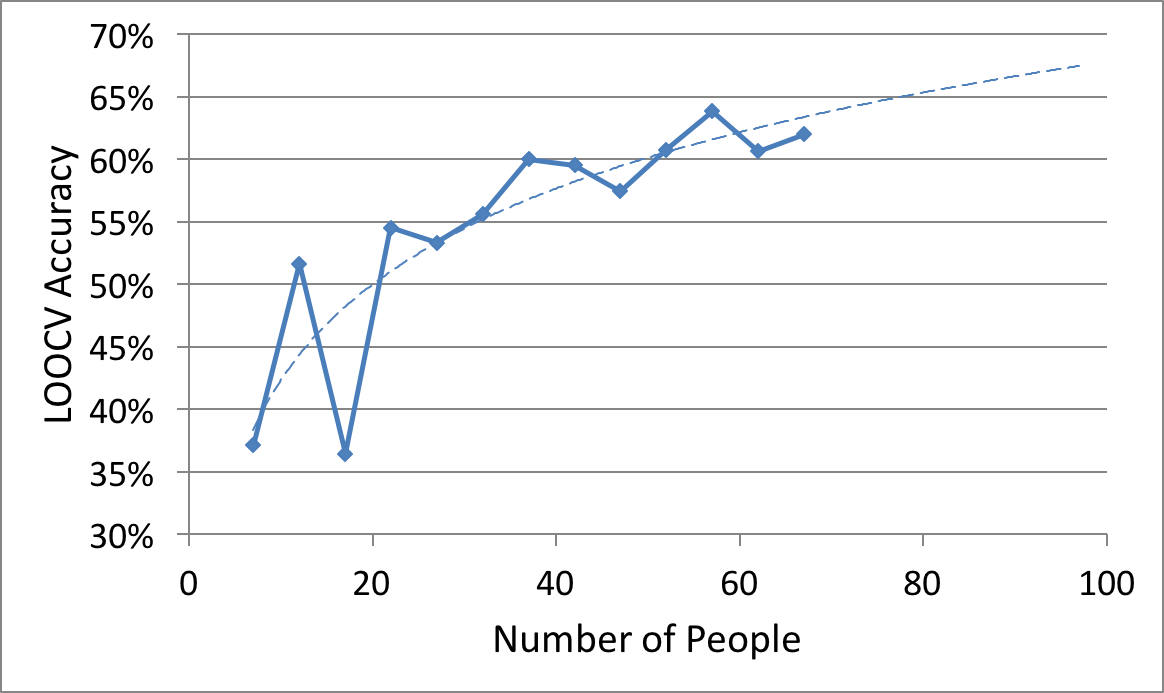
\includegraphics[width=.7\columnwidth,trim={0mm 0mm 0mm 0mm},clip]{Num_of_people_LOOCV}
        \vspace{-7pt}
        \caption[Effects of more people on prediction accuracy]{Effects of using more people for leave-one-out cross-validation.  As more people are included in the training data, the LOOCV accuracy of the classifier increases slowly.}
        \label{fig:people_generalization}
\end{figure}

Based on these analyses, it is clear that adding more people to an email dataset and adding people with more historial email data improved the accuracy of the job title classifier.

\section{Deep Learning Application}
Techniques such as random forests work well for small, low-dimensional data.
Deep learning is an emerging field that has proven to be very powerful and effective in solving very complex problems.
However, massive amounts of data are necessary to properly train a deep learning algorithm.
Unfortunately, data on that scale is unavailable for email analysis.
Consider a much larger dataset, made up of millions of people without labels.
In this case, a more sophisticated, deep learning model would be necessary for successful classification in order to accurately learn the complicated structure inherent to such large real-world datasets.
Suppose a representative sample of volunteers from the dataset self-identifies.
This would produce a set of labeled training data, transforming an unsupervised problem into to a semi-supervised one. 

A deep belief network (DBN) is one model used to solve these types of problems. 
A DBN is a generative graph with nodes that represent stochastic variables.
There are several layers of these nodes, some of which are visible and some of which are hidden.
Typically, the top two layers of nodes have undirected connections.
Therefore, these layers are actually Restricted Boltzman machines (RBMs).
The rest of the layers use directed edges, forming a Bayesian network.
An example DBN is shown in Figure~\ref{fig:DBN}.

\begin{figure}[t]
    \centering
        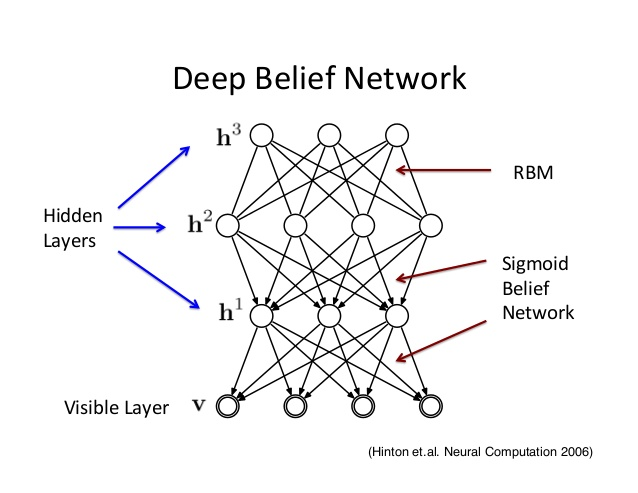
\includegraphics[width=.7\columnwidth,trim={0mm 0mm 0mm 0mm},clip]{dbn}
        \vspace{-7pt}
        \caption[The Components of a Deep Belief Network]{A deep belief network is a graphical network constructed by layering Restricted Boltzman machines on top of a Bayesian network~\cite{hinton_fast_2006}.}
        \label{fig:DBN}
\end{figure}

For the nodes in the Bayesian network layers, there exists a probability of activation, $p(s_i=1)$, which is represented by the nonlinear sigmoid function applied to a weighted input from the layer above.
Specifically,
\begin{equation}
p(s_i=1) = \frac{1}{1+\exp \left(-b_i-\sum_j s_j w_{ij}\right)}
\end{equation}
where $j$ represents the ancestors of node $i$, $w_{ij}$ are the weights on the connections between $i$ and $j$, and $b_i$ is the bias associated with node $i$.

The full DBN with $l$ hidden layers is able to model the joint distribution between inputs $x$ and those hidden layers:
\begin{equation}
P(x, h^1, ..., h^l) = \underbrace{\left(\prod_{k=0}^{l-2}P(h^k|h^{k+1}) \right)}_{\text{Bayesian network}} \underbrace{P(h^{l-1},h^l)}_{\text{RBM}}
\end{equation}

where $P(h^{l-1},h^l)$ represents the joint distribution of the top two layers, which form the RBM, and $x = h_0$.

The challenge with very deep networks is that training is very difficult and very time consuming~\cite{bengio_learning_2009}.
Unsupervised pre-training can improve the efficiency of training deep belief networks~\cite{hinton_recognize_2007}.
In that work, Hinton describes a fast, greedy method to train these networks one layer at a time.  This process is as follows:
\begin{enumerate}
\item Train an RBM on the input layer, $x$, and the first hidden layer, $h^1$.
\item Use the RBM to transform $x$ by sampling $p(h^1|h^0)$ or by finding the mean activations,\\ $p(h^1=1|h^0)$.
\item Repeat these steps up through the network until the top layer is reached.
\item Fine-tune all parameters of the deep network
\end{enumerate}

 
Testing on the MNIST dataset of handwritten digits, unsupervised pre-training is shown to improve classification results over only supervised training~\cite{erhan_why_2010}. 
Pre-training identifies a set of initial weights for the network that can ultimately lead to better classification results.  
An advantage of unsupervised pre-training is that, with small enough layers, it acts as a regularizer by decreasing variance and increasing the bias~\cite{hinton_recognize_2007}.  

In conjunction with greedy pre-training, backpropagation  with some labeled data has been shown to improve both the optimization and generalization of a DBN. 
Hinton et al. showed that unsupervised pre-training followed by backpropagation of a DBN outperformed traditional feed forward neural networks on the MNIST dataset~\cite{hinton_fast_2006}.
The nonlinearity of the logistic function used in backpropagation mitigates the possibility of overfitting to the data.

Much of the research in deep learning today is focused on image classification and analysis, such as the MNIST dataset.  However, DBNs have been applied to text analysis as well.
Ruangkanokmas et al. developed a sophisticated version of a DBN was used to construct a sentiment classifier~\cite{ruangkanokmas_deep}.
The purpose of that research was to label online reviews as positive, negative, or neutral.
The difference between this method and other DBN approaches is that this work replaced some of the hidden layers of the network with a feature selection step.
Overall, this improves the training efficiency of the algorithm.
This method can classify sentiments more accurately and train more quickly than previous semi-supervised algorithms.
A classifier such as this could be used to powerfully learn with extremely large email datasets, particularly those without hashed text.



\chapter{Conclusions} \label{Conclusions}
This work presents a new dataset, approximately the size of the Enron dataset, that was collected from volunteers' emails with particular attention to protect volunteers' privacy.
The new dataset includes accurate labels prepared by researchers with knowledge of the center and its employees.

A variety of features are calculated from this dataset and used with a random forest algorithm to automatically classify the center's employees.
This feature set includes features that had been studied in the past but also others that are unique to this data.
Furthermore, this research presents a list of features that combines the two previous schools of thought: traffic-based features and social-based features.

Random forests are shown to be powerful classifiers by predicting employee job titles with 96\% accuracy, even for employees for whom only secondhand data is available in the dataset.
The result showed an improved leave-one-out cross-validation error that surpasses previous work on the Enron corpus, using a dataset that has a fraction of the samples.
The email data was also used to show that emails could be used to predict an employee's primary program manager, but had a worse chance of being able to identify the director associated with the employee on the official organizational chart.

A method for generating an organic hierarchy was presented.
This chart could be a useful tool in aiding large corporate reorganizations by clearly summarizing project-based and social relationships not immediately evident from official records.
This work has shown that it is possible to glean organizational information from using carefully processed email metadata without compromising the email privacy of employees.


%
% Include an EPS figure with this command:
%   \epsffile{filename.eps}
%

%%%%%%%%%%%%%%%%
%
% Do tables like this:

% \begin{table}
% \caption{The Graduate School wants captions above the tables.}
%\begin{center}
% \begin{tabular}{ccc}
% x & 1 & 2 \\ \hline
% 1 & 1 & 2 \\
% 2 & 2 & 4 \\ \hline
% \end{tabular}
%\end{center}
% \end{table}

%%%%%%%%%%%%%%%%%%%%%%%%%%%%%%%%

\bibliographystyle{ieeetr}
\bibliography{bib}

\appendix

% In LaTeX, each appendix is a "chapter"
% \chapter{Program Source}
\chapter*{Appendix A: Example Email}
\lstinputlisting[language=email]{1439900489.txt}


\chapter*{Appendix B: Full Feature List}
\begin{enumerate}
	\setlength\itemsep{-0.75em}
	\item total\_sent
	\item unique\_addresses\_sent
	\item unique\_add\_sent\_perc
	\item unique\_subjects\_sent
	\item unique\_sub\_sent\_perc
	\item total\_received
	\item unique\_addresses\_received
	\item uniqueadd\_rec\_perc
	\item unique\_subjects\_received
	\item unique\_sub\_rec\_perc
	\item total\_emails
	\item total\_sent\_signed
	\item total\_sent\_signed\_perc
	\item unique\_addresses\_sent\_signed
	\item unique\_add\_sent\_perc\_signed
	\item unique\_subjects\_sent\_signed
	\item unique\_sub\_sent\_perc\_signed
	\item total\_received\_signed
	\item total\_rec\_signed\_perc
	\item unique\_addresses\_received\_signed
	\item unique\_add\_rec\_perc\_signed
	\item unique\_subjects\_received\_signed
	\item unique\_sub\_rec\_perc\_signed
	\item total\_sent\_encrypted
	\item total\_sent\_encrypted\_perc
	\item unique\_addresses\_sent\_encrypted
	\item unique\_add\_sent\_perc\_encrypted
	\item unique\_subjects\_sent\_encrypted
	\item unique\_sub\_sent\_perc\_encrypted
	\item total\_received\_encrypted
	\item total\_rec\_encrypted\_perc
	\item unique\_addresses\_received\_encrypted
	\item unique\_add\_rec\_perc\_encrypted
	\item unique\_subjects\_received\_encrypted
	\item unique\_sub\_rec\_perc\_encrypted
	\item inter\_hume\_sent
	\item inter\_hume\_received
	\item inter\_vt\_sent
	\item inter\_vt\_received
	\item sent\_to
	\item sent\_to\_perc
	\item sent\_cc
	\item sent\_cc\_perc
	\item rec\_to
	\item rec\_to\_perc
	\item rec\_cc
	\item rec\_cc\_perc
	\item avg\_recipients\_sent
	\item avg\_recipients\_rec
	\item avg\_body\_chars\_sent
	\item avg\_body\_chars\_rec
	\item var\_body\_chars\_sent
	\item var\_body\_chars\_rec
	\item after\_hours\_sent
	\item after\_hours\_sent\_perc
	\item after\_hours\_rec
	\item after\_hours\_rec\_perc
	\item after\_hours\_sent\_hume
	\item after\_hours\_sent\_hume\_perc
	\item after\_hours\_rec\_hume
	\item after\_hours\_rec\_hume\_perc
	\item avg\_sent\_per\_day
	\item avg\_rec\_per\_day
	\item avg\_emails\_per\_day
	\item attached\_sent
	\item attached\_rec
	\item avg\_attachments\_sent
	\item avg\_attachments\_rec
	\item sent\_re
	\item sent\_re\_perc
	\item sent\_fw
	\item sent\_fw\_perc
	\item rec\_re
	\item rec\_re\_perc
	\item rec\_fw
	\item rec\_fw\_perc
	\item avg\_subject\_chars\_sent
	\item avg\_subject\_chars\_rec
	\item var\_subject\_chars\_sent
	\item var\_subject\_chars\_rec
	\item fg\_between\_centrality
	\item pg\_between\_centrality
	\item pg\_avg\_neighbor\_degree
	\item fg\_avg\_neighbor\_degree
	\item pg\_clustering
	\item fg\_clustering
	\item pg\_closeness\_centrality
	\item fg\_closeness\_centrality
	\item pg\_degree\_centrality
	\item fg\_degree\_centrality
	\item pg\_current\_flow\_closeness\_centrality
    \item fg\_current\_flow\_closeness\_centrality
	\item pg\_current\_flow\_betweenness\_centrality
	\item fg\_current\_flow\_betweenness\_centrality
	\item pg\_communicability\_centrality
	\item fg\_communicability\_centrality
	\item pg\_communicability\_betweenness\_centrality
	\item fg\_communicability\_betweenness\_centrality
	\item pg\_load\_centrality
	\item fg\_load\_centrality
	\item pg\_square\_clustering
	\item fg\_square\_clustering
	\item fg\_eccentricity
	\item pg\_eccentricity
	\item pg\_pagerank
	\item fg\_pagerank
	\item pg\_hubs
	\item pg\_authorities
	\item fg\_hubs
	\item fg\_authorities
	\item pg\_avg\_shortest\_paths
	\item fg\_avg\_shortest\_paths
	\item pg\_num\_cliques
	\item fg\_num\_cliques
\end{enumerate}

\end{document}

